% Template LaTeX Tesis Ciencia de la Computación UCSP
% 2022

\documentclass[a4paper,openany,12pt]{book}
\usepackage[utf8]{inputenc}
\usepackage{graphicx}
\usepackage[spanish,mexico]{babel}
\usepackage{sty/fancyhdr}
\usepackage{ae}
\usepackage[left=2.5cm,right=2.5cm,top=3cm,bottom=2cm]{geometry}
\usepackage[printonlyused]{acronym}
\usepackage{xspace}
\usepackage{sty/hlundef}
\usepackage{sty/tesis}
\usepackage{setspace}
\usepackage{booktabs}
\usepackage{url}
\usepackage{float}
\usepackage{amsmath}
\usepackage{amssymb}
\usepackage{needspace}

% Penalizaciones máximas contra viudas y huérfanas (auditoría F1.4 / F1.5).
\widowpenalty=10000
\clubpenalty=10000

% Evita que un título de sección quede solo al pie de página.
\let\oldsection\section
\renewcommand{\section}{\needspace{6\baselineskip}\oldsection}
\let\oldsubsection\subsection
\renewcommand{\subsection}{\needspace{5\baselineskip}\oldsubsection}
\let\oldsubsubsection\subsubsection
\renewcommand{\subsubsection}{\needspace{4\baselineskip}\oldsubsubsection}


\title{Pipeline liviano para Action Quality Assessment basado en arquitecturas modernas de bajo costo computacional}

\author{Emmanuel Samir Galdos Rodriguez}


\advisor{Edward Jorge Yuri Cayllahua Cahuina}


\date{Arequipa, 2026}

%\examinerone{Prof. Dr. Hidalgo Buena Gente}{Presidente}%
%\examinertwo{Prof. Dr. Antero A. Gal Oppe}{Secretario}%
%\examinerthree{Prof. Dr. Liu Xiao Ling}{University of ...} % of being the case

\dedicado{A mi familia, por su apoyo constante a lo largo de este proceso.}

\begin{document}
\pagestyle{fancy}

\maketitle %Compone la carátula y la dedicatoria
\newpage

%\approved{\tres}%  {\tres} or {\cuatro}

%mayores detalles de como usas las abreviaturas (acronimos)
% vea: http://www.ctan.org/tex-archive/macros/latex/contrib/acronym/
% hay un manual en pdf en esa misma direccion

\chapter*{Abreviaturas}

\begin{acronym}
\acro{AQA}{\textit{Action Quality Assessment}}
\acro{KD}{\textit{Knowledge Distillation}}
\acro{I3D}{\textit{Inflated 3D ConvNet}}
\acro{TSM}{\textit{Temporal Shift Module}}
\acro{SRCC}{\textit{Spearman Rank Correlation Coefficient}}
\acro{PLCC}{\textit{Pearson Linear Correlation Coefficient}}
\acro{MAE}{\textit{Mean Absolute Error}}
\acro{FLOPs}{\textit{Floating Point Operations}}
\acro{CNN}{\textit{Convolutional Neural Network}}
\acro{RGB}{\textit{Red, Green, Blue}}
\acro{MSE}{\textit{Mean Squared Error}}
\acro{KL}{\textit{Kullback--Leibler}}
\end{acronym}


\begin{agradecimientos}
A mi familia, por el apoyo constante e incondicional brindado durante todos los años de formación universitaria.

A la Universidad Católica San Pablo, mi \textit{alma mater}, por la formación recibida y por el entorno académico que hizo posible este trabajo.

A mi asesor, Mg. Edward Jorge Yuri Cayllahua Cahuina, por su orientación, su paciencia y su guía rigurosa a lo largo del desarrollo de esta tesis.

A mis profesores y compañeros de la carrera de Ciencia de la Computación, por las discusiones, el aprendizaje compartido y los retos que motivaron este proyecto.
\end{agradecimientos}
 %Inserta los agradecimientos
\begin{resumen}
La Evaluación de la Calidad de Acciones (\textit{Action Quality Assessment}, AQA) en video tiene aplicaciones en deporte, rehabilitación y educación, pero los modelos de referencia (I3D, SlowFast) presentan un coste computacional prohibitivo para dispositivos con recursos limitados. Esta tesis aborda dos preguntas relacionadas: ¿en qué medida un \textit{pipeline} liviano basado en arquitecturas modernas puede aproximarse al rendimiento de un Teacher 3D profundo en AQA?, y ¿qué componentes del \textit{pipeline} sostienen ese rendimiento? Se propone un \textit{pipeline} reproducible basado en TSM-MobileNetV2 y MobileNetV3, inicializados con pesos preentrenados en ImageNet y entrenados con AdamW, programación cosenoidal, precisión mixta y acumulación de gradientes. La evaluación cubre tres dominios (AQA-7 multi-disciplina deportiva, MTL-AQA clavados, JIGSAWS cirugía robótica) y dos Teachers de referencia (I3D-R50 e SlowFast-R50). En AQA-7, el \textit{pipeline} liviano alcanza correlaciones SRCC de $0.9021 \pm 0.005$ (TSM-MobileNetV2) y $0.8907 \pm 0.005$ (MobileNetV3) sobre tres semillas, frente a $0.9052$ del I3D y $0.9158$ del SlowFast-R50; la brecha se mantiene menor a $0.025$ SRCC y robusta entre semillas, utilizando apenas $9\%$ de los FLOPs y reduciendo la latencia a 40~ms por clip. Las ablaciones identifican el preentrenamiento ImageNet ($\sim 3$ puntos SRCC) y el módulo Temporal Shift ($\sim 1$ punto adicional) como los componentes responsables del rendimiento. La transferencia cruzada delimita el alcance: MTL-AQA $\to$ AQA-7 transfiere parcialmente (SRCC $\sim 0.55$); AQA-7 $\to$ JIGSAWS fracasa. Como análisis marginal, se evalúa el aporte de la destilación de conocimiento sobre el \textit{pipeline} liviano; sólo 1 de 6 configuraciones mejora con destilación, lo cual cuestiona la premisa heredada de la literatura de que la destilación es necesaria para cerrar la brecha entre Teacher y Student. El código fuente, las configuraciones experimentales y los \textit{checkpoints} del \textit{pipeline} se publican como recurso reproducible.
\end{resumen}
 %Inserta el resumen
\begin{abstract}
Action Quality Assessment (AQA) busca cuantificar objetivamente la calidad de ejecución de acciones humanas en video, con aplicaciones en deporte, rehabilitación y educación. Los modelos de referencia se apoyan en arquitecturas 3D profundas (I3D, SlowFast) con alto coste computacional, lo que limita su uso en dispositivos con recursos limitados. Esta tesis aborda dos preguntas: (i) ¿en qué medida un \textit{pipeline} liviano basado en arquitecturas modernas (TSM-MobileNetV2, MobileNetV3), bien inicializado con pesos de ImageNet y entrenado con prácticas actuales (AdamW, cosine annealing, mixed precision, gradient accumulation), puede aproximarse al rendimiento de un Teacher 3D profundo?, y (ii) ¿qué componentes del \textit{pipeline} sostienen ese rendimiento, y dónde están sus límites de aplicabilidad?

Se propone un \textit{pipeline} reproducible aplicado a tres dominios de naturaleza distinta (AQA-7 multi-disciplina deportiva, MTL-AQA clavados especializados, JIGSAWS cirugía robótica), evaluado contra dos Teachers de referencia: I3D-R50 (referencia histórica) y SlowFast-R50 (referencia 3D moderna). En AQA-7, los Students livianos alcanzan SRCC de $0.9021 \pm 0.005$ (TSM-MobileNetV2) y $0.8907 \pm 0.005$ (MobileNetV3) sobre tres semillas, frente a $0.9052$ del I3D y $0.9158$ del SlowFast-R50, con brecha menor a $0.025$ SRCC y robusta entre semillas. Estos resultados utilizan sólo el $9\%$ de los FLOPs del Teacher I3D y reducen la latencia de inferencia a 40~ms por clip de 64 frames en una RTX 3060 Mobile. En MTL-AQA y JIGSAWS la brecha se mantiene menor a $0.01$ SRCC, confirmando estabilidad del \textit{pipeline} en dominios distintos.

Las ablaciones aíslan los componentes responsables del rendimiento: el preentrenamiento ImageNet aporta $\sim 0.031$ SRCC (sin él, el SRCC cae a $0.8713$) y el módulo Temporal Shift aporta $\sim 0.010$ SRCC adicional. Esto convierte el \textit{pipeline} en una propuesta interpretable, no en un efecto agregado opaco. La transferencia cruzada confirma límites: MTL-AQA $\to$ AQA-7 transfiere parcialmente (SRCC $\sim 0.55$); AQA-7 $\to$ JIGSAWS fracasa, delimitando el alcance del enfoque. Como análisis marginal de la destilación de conocimiento, se evalúa la variante \textit{+~KD} con pérdidas auxiliares de atención y alineación temporal; sólo 1 de 6 configuraciones (MobileNetV3 + AQA-7) mejora con destilación, mientras que las restantes degradan, en algunos casos de forma severa. Este resultado cuestiona la premisa heredada de la literatura de que la destilación es necesaria para cerrar la brecha entre Teacher y Student livianos. El código fuente, las configuraciones experimentales y los \textit{checkpoints} se publican como recurso reproducible.
\end{abstract}
 %Inserta el abstract

\pagenumbering{roman}
\setcounter{page}{1}
\pagestyle{plain}

\tableofcontents %Inserta el índice general
\listoftables %Inserta el índice de cuadros
\listoffigures %Inserta el índice de figuras



%%%%%%%%%%%%%%%%%%%%%%%%%%%%%%%%%%%%%%%%%%%%%%%%%%%%%%%%%%%%%%%%%%%%%
%%%%   En esta parte deberas incluir los archivos de tu tesis   %%%%%
%%%%%%%%%%%%%%%%%%%%%%%%%%%%%%%%%%%%%%%%%%%%%%%%%%%%%%%%%%%%%%%%%%%%%

\pagestyle{plain}
\pagenumbering{arabic}
\setcounter{page}{1}
\chapter{Introducción}

\section{Motivación y Contexto}

En los últimos años, el reconocimiento automático de acciones humanas en video ha emergido como un área clave dentro del campo de la visión por computadora, con aplicaciones que abarcan desde la seguridad y el entretenimiento hasta la medicina y el deporte. Más allá de identificar qué acción se realiza en un video, ha cobrado relevancia una tarea más compleja: la \textbf{Evaluación de la Calidad de Acciones} (\textit{Action Quality Assessment}, \ac{AQA}). Esta disciplina busca medir la calidad con la que se ejecuta una acción, considerando criterios como la técnica, la fluidez y la precisión del movimiento. A diferencia del reconocimiento de acciones, \ac{AQA} introduce desafíos adicionales tanto en términos de modelado como de evaluación.

El interés por \ac{AQA} ha crecido sustancialmente debido a su potencial impacto en contextos donde el desempeño técnico es crítico. En el ámbito deportivo, entrenadores y atletas pueden aprovechar sistemas automáticos para recibir retroalimentación objetiva y detallada que complemente la evaluación humana. En rehabilitación física, los profesionales podrían beneficiarse de modelos que evalúen en tiempo real la correcta ejecución de ejercicios terapéuticos, facilitando el seguimiento remoto de pacientes. En educación médica, la evaluación automática de gestos quirúrgicos podría apoyar la formación de residentes.

A pesar de estos beneficios potenciales, uno de los principales obstáculos para la adopción de sistemas de \ac{AQA} en escenarios reales radica en su elevada demanda computacional. Modelos de alto rendimiento basados en arquitecturas tridimensionales profundas, como I3D \cite{Carreira2017I3D} y SlowFast \cite{feichtenhofer2019slowfast}, han demostrado alta precisión al capturar patrones espacio-temporales complejos. Sin embargo, su tamaño y costo computacional los hacen inviables para aplicaciones que requieren baja latencia, eficiencia energética o procesamiento local en dispositivos con recursos limitados.

\section{Planteamiento del Problema}

La estimación automática de la calidad de acciones en video requiere capturar información espacial y temporal asociada a la ejecución de una acción humana. Los modelos 3D profundos, como \ac{I3D}, han sido ampliamente utilizados por su capacidad para modelar dependencias espacio-temporales complejas; sin embargo, su alto costo computacional limita su uso en escenarios donde se requiere baja latencia, menor consumo de memoria o despliegue en dispositivos con recursos limitados.

La literatura reciente ha propuesto la destilación de conocimiento (\textit{Knowledge Distillation}, \ac{KD}) \cite{Hinton2015Distilling} como estrategia para transferir información desde modelos \textit{Teacher} pesados hacia modelos \textit{Student} livianos. Esta línea de trabajo \cite{Yu2021GroupAware,Mun2019TKD,Cai2023VisionLanguageAQA} parte de la premisa de que las arquitecturas livianas presentan una brecha sustancial de rendimiento frente al \textit{Teacher} y que dicha brecha debe cerrarse mediante señales adicionales de supervisión. No obstante, esta premisa fue formulada en un contexto donde los pesos preentrenados disponibles, las prácticas de entrenamiento y las arquitecturas eficientes eran menos maduras.

Actualmente, los modelos livianos pueden beneficiarse de pesos modernos preentrenados en ImageNet, optimizadores como AdamW, programación cosenoidal de la tasa de aprendizaje, entrenamiento con precisión mixta, acumulación de gradientes y módulos temporales eficientes como \textit{Temporal Shift Module} \cite{Lin2019TSM}. Bajo este nuevo escenario, no está claro si los \textit{Students} livianos siguen requiriendo destilación para aproximarse al rendimiento de un \textit{Teacher} 3D, ni cuáles son los límites reales de un \textit{pipeline} liviano moderno para \ac{AQA}.

A partir de esta problemática, surge la siguiente \textbf{pregunta de investigación}:

\begin{quote}
\textbf{¿En qué medida un \textit{pipeline} liviano basado en arquitecturas modernas (TSM-MobileNetV2 y MobileNetV3), correctamente inicializado y entrenado con prácticas actuales, puede aproximarse al rendimiento de un \textit{Teacher} 3D profundo en \ac{AQA} a un costo computacional sustancialmente menor, y dónde están sus límites de aplicabilidad?}
\end{quote}

Este trabajo aborda dicho problema mediante el desarrollo de un \textit{pipeline} eficiente basado en arquitecturas livianas modernas, evaluando su capacidad para aproximarse al rendimiento de \ac{I3D} y \textit{SlowFast} en distintos dominios, caracterizando su costo computacional y delimitando los escenarios donde el enfoque resulta suficiente o requiere mecanismos adicionales.

\section{Objetivos}

\subsection{Objetivo General}

Desarrollar un \textit{pipeline} eficiente de \textit{Action Quality Assessment} basado en arquitecturas livianas modernas, evaluando empíricamente su capacidad para alcanzar rendimiento competitivo respecto a modelos 3D profundos en dominios de naturaleza distinta y delimitando sus límites de aplicabilidad.

\subsection{Objetivos Específicos}

\begin{itemize}
  \item \textbf{OE1.} Revisar el estado del arte en \ac{AQA} y métodos de compresión o destilación aplicados a video, identificando las principales suposiciones sobre la brecha entre modelos \textit{Teacher} 3D y \textit{Students} livianos.

  \item \textbf{OE2.} Construir un \textit{pipeline} reproducible de entrenamiento e inferencia para \textit{Students} livianos, específicamente \ac{TSM}-MobileNetV2 y MobileNetV3, empleando pesos preentrenados, optimización moderna, precisión mixta y acumulación de gradientes.

  \item \textbf{OE3.} Cuantificar la brecha de rendimiento entre los \textit{Students} livianos y el \textit{Teacher} \ac{I3D} mediante \ac{SRCC}, \ac{PLCC} y \ac{MAE} en datasets representativos de \ac{AQA}, complementando la comparación con un \textit{Teacher} 3D más moderno (SlowFast-R50) en el dataset principal.

  \item \textbf{OE4.} Analizar el impacto de componentes clave del \textit{pipeline} mediante ablaciones mínimas sobre el dataset principal, priorizando las decisiones con mayor efecto esperado en el rendimiento (preentrenamiento ImageNet y módulo temporal).

  \item \textbf{OE5.} Caracterizar la eficiencia computacional del \textit{pipeline} propuesto en términos de parámetros, \ac{FLOPs} y latencia de inferencia frente al \textit{Teacher} \ac{I3D}.

  \item \textbf{OE6.} Delimitar los límites de aplicabilidad del \textit{pipeline} mediante análisis complementarios de transferencia cruzada entre dominios y aporte marginal de la destilación de conocimiento sobre la línea base liviana.
\end{itemize}

\section{Organización de la Tesis}
\label{sec:organizacion}

El presente documento está estructurado de la siguiente manera:

\begin{itemize}
    \item \textbf{Capítulo 2: Marco Teórico} -- Fundamentos de \textit{Action Quality Assessment} (\ac{AQA}), métricas clave (\ac{SRCC}, \ac{PLCC}, \ac{MAE}), conjuntos de datos (AQA-7, MTL-AQA, JIGSAWS) y nociones de \ac{KD}.

    \item \textbf{Capítulo 3: Estado del Arte} -- Revisión de técnicas recientes en \ac{AQA} y \ac{KD} aplicada a video, con énfasis en las suposiciones sobre la brecha entre \textit{Teacher} y \textit{Student}.

    \item \textbf{Capítulo 4: Propuesta} -- Metodología completa del \textit{pipeline} liviano: arquitecturas \textit{Student} (\ac{TSM}-MobileNetV2 y MobileNetV3), receta de entrenamiento moderna, datasets y protocolo de evaluación. Se incluye también el módulo de destilación que se utiliza como análisis marginal en el Capítulo 5.

    \item \textbf{Capítulo 5: Resultados} -- Comparación principal del \textit{pipeline} liviano frente a los \textit{Teachers} \ac{I3D} y SlowFast-R50, ablaciones sobre el preentrenamiento ImageNet y el módulo temporal, eficiencia computacional, transferencia cruzada y análisis marginal de la destilación.

    \item \textbf{Capítulo 6: Conclusiones} -- Hallazgos clave alineados a los objetivos específicos, limitaciones y direcciones futuras.
\end{itemize}
 %Inserta el capítulo 1








%NUeva estructuracion%

\chapter{Marco Teórico}\label{chap:background}

En este capítulo se exponen los fundamentos teóricos necesarios para comprender la evaluación de la calidad de acciones (\ac{AQA}) y la distilación de conocimiento (\ac{KD}) en el contexto de visión por computador. Se abordan las definiciones, desafíos inherentes, métricas de evaluación y estructuras arquitectónicas clave que sustentan la propuesta metodológica desarrollada en esta tesis.

\section{Evaluación de la Calidad de Acciones}

\subsection{Definición y desafíos}

La \ac{AQA} tiene como objetivo cuantificar objetivamente la calidad de ejecución de acciones humanas capturadas en video. A diferencia de las tareas tradicionales de clasificación de acciones, donde se identifica qué acción se realiza, en \ac{AQA} se mide la competencia, técnica, fluidez y precisión con que se realiza dicha acción \cite{Zhou2025Survey}. Esta característica hace que la tarea sea particularmente exigente, pues implica una comprensión profunda del contenido visual y de las dinámicas temporales.

\subsubsection{Limitaciones de los conjuntos de datos}

\paragraph{Escasez de muestras y desequilibrio.}
Los conjuntos de datos disponibles en AQA tienden a ser específicos de dominios muy concretos, como el clavado olímpico o la gimnasia artística. Esto conlleva una limitada diversidad de escenarios y una reducida cantidad de ejemplos etiquetados, lo cual complica el aprendizaje generalizable \cite{WangAQA2019}. Además, las etiquetas de calidad suelen distribuirse de forma sesgada, con acumulaciones en puntajes medios, lo que penaliza la capacidad de los modelos para identificar instancias en los extremos de calidad \cite{Wang2024Review}.

\paragraph{Anotaciones subjetivas.}
Las etiquetas suelen derivarse de la evaluación humana, típicamente por jueces expertos. Esta subjetividad introduce variabilidad y ruido en las etiquetas. Técnicas como el coeficiente $\kappa$ de Cohen o la correlación interevaluador se utilizan para medir consistencia, pero el proceso sigue siendo costoso y propenso a sesgos \cite{Li2019ActionEval}.

\paragraph{Generalización y adaptabilidad.}
Los modelos tienden a especializarse en un dominio específico y fallan al generalizar a nuevos tipos de acción o entornos sin un proceso de reentrenamiento. Las estrategias de aprendizaje multitarea y adaptación de dominio han mostrado avances limitados en este aspecto \cite{Parmar2019MTLAQA}.

\subsubsection{Retos computacionales}

\paragraph{Complejidad espacio–temporal.}
Capturar dependencias espaciales y temporales de forma conjunta exige arquitecturas profundas que trabajen con secuencias completas. Modelos como \ac{I3D} operan con convoluciones 3D que implican un alto costo computacional y grandes requerimientos de memoria \cite{Carreira2017I3D}.

\paragraph{Latencia y tiempo real.}
La evaluación de calidad en tiempo real es relevante para aplicaciones móviles o sistemas de retroalimentación inmediata. Modelos livianos como \ac{TSM} o MobileNet-V3 sacrifican parte de su precisión para lograr una menor latencia de inferencia, lo que plantea un desafío al balancear velocidad y exactitud \cite{Howard2019MobileNetV3,Wang2024Review}.

\subsubsection{Variabilidad intra‐clase}

Acciones de la misma categoría pueden diferir en estilo, velocidad, o incluso en perspectiva de grabación. Esta variabilidad intra-clase dificulta la generación de representaciones robustas que capten la esencia de lo que constituye una ejecución “de calidad”. Un ejemplo claro se da en los clavados olímpicos, donde ejecuciones técnicamente distintas pueden ser igualmente válidas, dependiendo del estilo del atleta \cite{Pirsiavash2014AssessedQuality,Yu2021GroupAware}.

\subsection{Datasets y métricas}

En la Tabla~\ref{tab:aqa_datasets} se enumeran los principales datasets empleados en tareas de \ac{AQA}, destacando su dominio de aplicación, la escala de puntuación y las métricas de evaluación.

Las métricas más utilizadas incluyen:

\begin{itemize}
    \item \textbf{SRCC (Spearman Rank Correlation Coefficient)}: mide la correlación entre el orden de las predicciones y las etiquetas reales.
    \item \textbf{PLCC (Pearson Linear Correlation Coefficient)}: evalúa la relación lineal entre puntuaciones predichas y reales.
    \item \textbf{MAE (Mean Absolute Error)}: cuantifica el error promedio absoluto entre predicción y verdad de terreno.
\end{itemize}

\begin{table}[ht]
    \centering
    \caption{Principales datasets empleados en \ac{AQA}.}
    \label{tab:aqa_datasets}
    \begin{tabular}{|l|c|p{8.5cm}|}
    \hline
    \textbf{Dataset} & \textbf{Año} & \textbf{Descripción y métricas} \\
    \hline
    MIT-Diving & 2014 & 370 videos de clavados olímpicos, puntuación humana [0–100], métricas: SRCC, PLCC, MAE \cite{Pirsiavash2014AssessedQuality}. \\
    \hline
    UNLV-Vault & 2018 & 176 videos de salto de gimnasia, puntuaciones [0–20], SRCC, MAE \cite{Wang2022AQASurvey}. \\
    \hline
    AQA-7 & 2017 & 1 189 videos de siete deportes (clavados, gimnasia, esquí, etc.), anotaciones detalladas, SRCC, PLCC, MAE \cite{Parmar2017AQA7}. \\
    \hline
    MTL-AQA & 2019 & 1 412 videos de clavados (plataforma y trampolín), clasificación multietiqueta y regresión de puntuación \cite{Parmar2019MTLAQA}. \\
    \hline
    JIGSAWS & 2013 & Videos de suturas quirúrgicas, métricas de precisión de movimiento para AQA en cirugía robótica \cite{DiPietro2013JIGSAWS}. \\
    \hline
    \end{tabular}
\end{table}

\section{Distilación de Conocimiento}

\subsection{Principios y variantes}

La distilación de conocimiento (\ac{KD}) permite transferir información desde un modelo complejo y de alto rendimiento (Teacher) a un modelo más pequeño y eficiente (Student), con el objetivo de preservar la mayor cantidad de conocimiento posible. Esta técnica ha demostrado ser eficaz tanto en tareas de clasificación como de regresión, especialmente cuando se desea desplegar modelos en entornos con restricciones de cómputo \cite{Hinton2015Distilling}.

Los principales enfoques de distilación son:

\begin{itemize}
  \item \textbf{Offline:} el Teacher se entrena previamente y sus parámetros permanecen fijos durante el proceso de distilación.
  \item \textbf{Online:} Teacher y Student se entrenan simultáneamente, permitiendo una interacción dinámica entre ambos.
  \item \textbf{Self-distillation:} distintos componentes de un mismo modelo actúan como Teacher y Student, transfiriendo internamente conocimiento entre capas o cabezas \cite{Sarkar2022XKD}.
\end{itemize}

\subsection{Distilación en visión por video}

Aplicar \ac{KD} en videos requiere considerar el componente temporal, además del espacial. En este contexto, se han desarrollado diversas estrategias, tales como:

\begin{itemize}
  \item \textbf{Transferencia de mapas de atención:} el Student es guiado para replicar las regiones espacio-temporales en las que el Teacher focaliza su atención \cite{Yu2021GroupAware}.
  \item \textbf{Alineación temporal:} sincronización de representaciones generadas por el Teacher y el Student en cada paso temporal, preservando patrones de movimiento \cite{Mun2019TKD}.
  \item \textbf{Multimodalidad:} destilar conocimiento desde múltiples modalidades (RGB, flujo óptico, audio) hacia un Student que trabaja con una sola entrada, comúnmente RGB \cite{Cai2023VisionLanguageAQA}.
\end{itemize}

Cada una de estas variantes busca mantener la fidelidad de las representaciones aprendidas por el Teacher, al tiempo que reduce los costos de inferencia y despliegue. En capítulos posteriores se examinará cómo estas estrategias se pueden aplicar específicamente a la evaluación de calidad de acciones.

\chapter{Estado del Arte}\label{chap:sota}

En este capítulo se analizan los avances recientes en la aplicación de técnicas de distilación de conocimiento en la tarea de evaluación de la calidad de acciones (\ac{AQA}). Se destacan tanto las estrategias arquitectónicas como las innovaciones metodológicas que han permitido mejorar la eficiencia y generalización de los modelos en este dominio.

\section{Distilación en AQA: avances recientes}

El uso de distilación de conocimiento en AQA ha ganado atención por su capacidad de reducir la complejidad de modelos sin sacrificar precisión, lo cual resulta especialmente útil dada la escasez de datos anotados y la naturaleza computacionalmente intensiva de los modelos espacio-temporales.

\subsection{Distilación intermodal: de múltiples flujos a RGB}

La distilación intermodal busca transferir conocimiento desde modelos complejos que procesan múltiples modalidades de entrada (como RGB, flujo óptico y articulaciones 3D) hacia modelos más simples que utilizan una sola modalidad, típicamente RGB. Este enfoque permite conservar la capacidad de razonamiento temporal y espacial sin requerir múltiples entradas durante la inferencia, lo cual es crucial para aplicaciones en tiempo real y dispositivos con recursos limitados.

Yu et al.~\cite{Yu2021GroupAware} proponen una estrategia denominada \textit{Group-Aware Knowledge Distillation} (GAKD), donde un modelo \textit{teacher} basado en múltiples flujos entrena a un modelo \textit{student} que opera únicamente sobre flujo RGB. Esta transferencia se realiza mediante una combinación de técnicas de distilación que incluyen:

\begin{itemize}
    \item \textbf{Distilación basada en atención espacial-temporal}: Se transfiere la atención del \textit{teacher} al \textit{student}, permitiendo que este último enfoque su atención en regiones y momentos clave de la secuencia de video.
    \item \textbf{Distilación de activaciones intermedias}: Se alinean las activaciones de capas intermedias entre el \textit{teacher} y el \textit{student}, facilitando que el \textit{student} aprenda representaciones jerárquicas similares.
    \item \textbf{Distilación de puntuaciones finales}: Se ajusta la salida final del \textit{student} para que coincida con la del \textit{teacher}, mejorando la precisión de las predicciones.
\end{itemize}

Además, GAKD incorpora un mecanismo de regresión contrastiva consciente de grupos (\textit{Group-aware Contrastive Regression}), donde se agrupan videos con atributos compartidos (como categoría y dificultad) y se aprende a predecir puntuaciones relativas entre ellos. Este enfoque reformula la evaluación de calidad de acciones como una tarea de comparación de pares, lo que ayuda a reducir la variabilidad en las puntuaciones y mejora la discriminación entre acciones similares.

Evaluado sobre el conjunto de datos AQA-7, GAKD logra un aumento significativo en la correlación de Spearman en comparación con modelos unimodales no distilados, estableciendo un nuevo estado del arte en esta tarea. Estos resultados demuestran la efectividad de la distilación intermodal para mejorar el rendimiento de modelos ligeros sin incrementar su complejidad computacional.



\subsection{Auto-distilación con supervisión multiescalar}

La auto-distilación con supervisión multiescalar es una estrategia emergente en la evaluación automatizada de la calidad de acciones (AQA), que busca mejorar la eficiencia y generalización de los modelos sin depender de un \textit{teacher} externo. Zhou et al.~\cite{Zhou2023AQA_SD} introducen el modelo \textit{Self-Distilled AQA}, que emplea una arquitectura híbrida CNN-Transformer para capturar patrones espacio-temporales jerárquicos de manera eficiente.

\paragraph{Arquitectura híbrida CNN-Transformer.} El modelo combina las capacidades de las redes convolucionales (CNN) para extraer características locales detalladas con la habilidad de los Transformers para modelar dependencias a largo plazo en secuencias temporales. Esta combinación permite una representación más rica y contextualizada de las acciones humanas, esencial para tareas de AQA donde tanto los detalles locales como la dinámica global son críticos.

\paragraph{Supervisión multiescalar interna.} Una característica distintiva de \textit{Self-Distilled AQA} es su mecanismo de auto-distilación interna. En lugar de requerir un modelo \textit{teacher} separado, el modelo utiliza sus propias capas profundas como supervisores para las capas más superficiales. Se implementa una función de pérdida multiescalar que alinea las representaciones generadas en diferentes niveles de la red, promoviendo la coherencia y consistencia entre las distintas escalas de representación. Este enfoque se inspira en trabajos previos que han demostrado los beneficios de la auto-distilación en redes neuronales profundas~\cite{zhang2019be}.

\paragraph{Eficiencia y despliegue.} Al eliminar la necesidad de un \textit{teacher} externo, el modelo reduce significativamente los costos computacionales y de almacenamiento asociados al entrenamiento y despliegue. Esta eficiencia lo hace particularmente adecuada para aplicaciones en dispositivos con recursos limitados, como sistemas móviles o embebidos, donde la capacidad de procesamiento y memoria es restringida.

\paragraph{Resultados empíricos.} En evaluaciones realizadas sobre los conjuntos de datos AQA-7 y UNLV-Vault, que incluyen tareas como clavados y salto de viga, \textit{Self-Distilled AQA} logra un rendimiento comparable al de modelos más complejos como I3D y SlowFast, pero con una reducción de hasta el 50\% en el número de parámetros. Estos resultados destacan la efectividad del enfoque en términos de precisión y eficiencia, posicionándolo como una solución viable para aplicaciones prácticas de AQA.

\paragraph{Perspectivas futuras.} La auto-distilación con supervisión multiescalar abre nuevas posibilidades para el desarrollo de modelos más compactos y generalizables en AQA. Su capacidad para integrar información jerárquica sin depender de supervisión externa lo convierte en un candidato prometedor para escenarios donde los datos etiquetados son escasos o costosos de obtener.


\subsection{Distilación multimodal \textit{vision--language}}

Un enfoque emergente en la distilación de conocimiento para AQA es la integración de señales provenientes de modalidades visuales y lingüísticas. Este paradigma se basa en la premisa de que las descripciones textuales de acciones humanas pueden aportar información semántica rica y complementaria a las representaciones visuales, especialmente en contextos donde los datos anotados manualmente son escasos o costosos de obtener.

Cai et al.~\cite{Cai2023VisionLanguageAQA} proponen un marco en dos etapas que aprovecha este principio. En la primera etapa, se entrena un modelo \textit{vision--language} sobre un corpus no supervisado utilizando aprendizaje contrastivo: se optimiza la similitud entre videos y sus correspondientes descripciones en lenguaje natural, incentivando que el modelo capture aspectos semánticamente relevantes del contenido visual (por ejemplo, ``clavado con entrada limpia y buena forma'' o ``fallo al girar completamente''). Este modelo actúa como \textit{teacher} multimodal, y su conocimiento es transferido a un \textit{student} unimodal (solo RGB) en la segunda etapa mediante distilación.

Durante el proceso de distilación, se aplican pérdidas auxiliares que alinean las representaciones latentes del student con aquellas generadas por el teacher \textit{vision--language}, sin necesidad de utilizar las descripciones textuales durante la inferencia. Esto permite que el student incorpore nociones semánticas complejas —como atributos estilísticos, errores técnicos o intenciones de la acción— sin depender de anotaciones explícitas al momento de la evaluación.

Los resultados reportados en~\cite{Cai2023VisionLanguageAQA} muestran mejoras significativas en la capacidad del student para generalizar hacia dominios no vistos (p.~ej., deportes o tipos de acción distintos a los del entrenamiento), así como una mayor robustez frente a variaciones en ángulos de cámara o estilo de ejecución. Este enfoque representa una dirección prometedora hacia modelos más interpretables y adaptables en AQA, al permitir que el conocimiento lingüístico actúe como un puente semántico para la representación visual.

Además, el uso de técnicas \textit{vision--language} abre nuevas posibilidades para el aprendizaje con pocos datos (\textit{few-shot learning}) y la transferencia de conocimiento desde dominios ampliamente etiquetados (como los usados en modelos tipo CLIP) hacia escenarios especializados como la evaluación técnica en deportes o cirugía asistida por robot.


\subsection{Distilación temporal con alineación dinámica}

Otra línea de investigación relevante en la distilación de conocimiento para AQA se centra en la dimensión temporal de las representaciones. A diferencia de enfoques tradicionales que distilan conocimiento sobre características agregadas (como el promedio de activaciones), las técnicas de distilación temporal buscan preservar la estructura secuencial de las acciones, capturando mejor los patrones de movimiento y transiciones clave a lo largo del tiempo.

Mun et al.~\cite{Mun2019TKD} introducen un método denominado \textit{temporal knowledge distillation} (TKD), en el cual se entrena al \textit{student} para que imite dinámicamente las representaciones del \textit{teacher} en cada instante de tiempo, permitiendo una alineación más fina entre las señales internas de ambos modelos. Para lograrlo, el método incorpora una pérdida de distilación calculada sobre las secuencias completas de activaciones, en lugar de solo comparar vectores promedio. Además, se utilizan técnicas de alineación dinámica (como Dynamic Time Warping) para manejar posibles desincronizaciones en la ejecución de las acciones, lo que resulta especialmente importante en contextos donde la duración o el ritmo de las secuencias puede variar entre muestras.

Este tipo de distilación resulta particularmente valioso en tareas de AQA donde la calidad de ejecución depende de la fluidez, consistencia y coordinación del movimiento a lo largo del tiempo. Por ejemplo, en disciplinas como clavados, patinaje artístico o rutinas gimnásticas, pequeñas variaciones temporales pueden implicar diferencias sustanciales en la puntuación otorgada por los jueces. Preservar estas características temporales permite al modelo estudiante capturar mejor los matices técnicos que afectan la calidad percibida de la acción.

En sus experimentos sobre el conjunto de datos MTL-AQA, Mun et al.~demuestran que el enfoque TKD mejora significativamente el coeficiente de correlación por rangos de Spearman (SRCC), indicando una mejor concordancia entre las predicciones del modelo y las puntuaciones reales. Cabe destacar que estas mejoras se logran sin necesidad de aumentar la cantidad de datos ni recurrir a arquitecturas más complejas, lo que evidencia la eficiencia del enfoque desde el punto de vista del entrenamiento.

Este tipo de distilación temporal abre nuevas posibilidades para capturar dinámicas complejas en modelos compactos y eficientes, y puede combinarse con otras estrategias (como distilación espacial o multimodal) para obtener representaciones más ricas y generalizables.


\section{Síntesis y brechas detectadas}

La Tabla~\ref{tab:aqa_kd_summary} resume los enfoques más representativos que han aplicado distilación de conocimiento en el contexto de AQA, detallando la modalidad de entrada, el tipo de distilación, y sus principales contribuciones.

\begin{table}[ht]
    \centering
    \caption{Resumen de trabajos relevantes en distilación aplicada a AQA.}
    \label{tab:aqa_kd_summary}
    \begin{tabular}{|p{3.5cm}|p{2.2cm}|p{2.8cm}|p{4.2cm}|}
    \hline
    \textbf{Trabajo} & \textbf{Entrada Student} & \textbf{Tipo de distilación} & \textbf{Contribuciones principales} \\
    \hline
    Yu et al. (2021) & RGB & Intermodal multistream & Distilación desde flujo óptico y pose 3D hacia RGB. Mejora en AQA-7. \\
    \hline
    Zhou et al. (2023) & RGB & Self-distillation jerárquica & Supervisión interna multiescalar, arquitectura eficiente para dispositivos móviles. \\
    \hline
    Cai et al. (2024) & RGB & Multimodal (vision–language) & Distilación de modelos contrastivos vision–language hacia evaluadores de calidad. \\
    \hline
    Mun et al. (2019) & RGB & Temporal dinámica & Preserva patrones secuenciales mediante alineación temporal en la distilación. \\
    \hline
    \end{tabular}
\end{table}

A pesar de los avances, persisten importantes desafíos:

\begin{itemize}
  \item \textbf{Escasa generalización} a dominios no deportivos o con acciones más cotidianas.
  \item \textbf{Falta de benchmark estandarizado} para comparar métodos de distilación en AQA.
  \item \textbf{Subaprovechamiento de modelos ligeros} como estudiantes en entornos de bajo cómputo.
\end{itemize}

En el próximo capítulo se presenta la metodología propuesta en esta tesis, que busca abordar parte de estas limitaciones mediante una estrategia de distilación adaptada al dominio AQA y orientada a modelos eficientes.
 %Inserta el capítulo 2
\chapter{Propuesta}
\label{cap:propuesta}
Este capítulo detalla la metodología propuesta: un \textit{pipeline} liviano para \textit{Action Quality Assessment} basado en arquitecturas modernas de bajo costo computacional. La propuesta se centra en dos componentes esenciales: (i) la elección de \textit{Students} livianos modernos (\ac{TSM}-MobileNetV2 y MobileNetV3) inicializados con pesos preentrenados en ImageNet, y (ii) una receta de entrenamiento moderna (AdamW, programación cosenoidal, precisión mixta, acumulación de gradientes) coherente con el preprocesamiento del \textit{Teacher} \ac{I3D}. Sobre esta línea base se evalúa, como análisis marginal en el Capítulo~\ref{chap:resultados}, un esquema de destilación de conocimiento (\ac{KD}) con el objetivo de cuantificar su aporte real cuando la línea base ya es fuerte.

% ---
\section{Planteamiento de la solución}

La hipótesis del trabajo es que los \textit{Students} livianos preentrenados en ImageNet, al combinar un \textit{pipeline} moderno de entrenamiento con un preprocesamiento coherente con el \textit{Teacher} (mismas estadísticas de Kinetics-400, misma longitud de clip $T=64$ a 25~FPS, mismas transformaciones espaciales), pueden cubrir la mayor parte de la brecha de rendimiento respecto al \textit{Teacher} \ac{I3D} sin necesidad de mecanismos adicionales. La validación empírica de esta hipótesis es la contribución central de la tesis.

El \textit{pipeline} propuesto se compone de los siguientes elementos, descritos en detalle en las secciones siguientes:

\begin{enumerate}
    \item Arquitecturas \textit{Student} livianas (Sección~\ref{sec:modelos}).
    \item Pérdida de regresión $\mathcal{L}_{reg}$ sobre la etiqueta de calidad.
    \item Receta de entrenamiento moderna: AdamW, cosine annealing, AMP, gradient accumulation (Sección~\ref{sec:evaluacion}).
    \item \textit{Pipeline} de datos uniforme para los tres dominios evaluados (Sección~\ref{sec:datasets}).
    \item Protocolo de evaluación con métricas de precisión y eficiencia computacional (Sección~\ref{sec:evaluacion}).
\end{enumerate}

\subsection{Función de pérdida principal}

El \textit{Student} se entrena con la pérdida de regresión sobre la puntuación normalizada $y \in [0, 1]$:

\[
\mathcal{L}_{reg}(\hat{y}, y) = \frac{1}{N} \sum_{i=1}^{N} (\hat{y}_i - y_i)^2,
\]

donde $\hat{y}$ es la predicción del \textit{Student} y $y$ la etiqueta real. Esta pérdida es suficiente para sostener la contribución central del trabajo. Los Capítulos~\ref{chap:resultados} y la Sección~\ref{sec:kd_marginal} evalúan, como análisis complementario, el aporte de pérdidas adicionales de destilación.

\subsection{Análisis marginal de la destilación}
\label{sec:kd_marginal}

Para responder \textbf{OE6} sobre la necesidad real del \ac{KD} cuando se dispone de un \textit{pipeline} liviano fuerte, se considera además un esquema de destilación con dos pérdidas auxiliares aplicadas durante el entrenamiento del \textit{Student}:

\begin{itemize}
    \item \textbf{Destilación de atención espacio-temporal ($\mathcal{L}_{att}$)}: se extraen mapas de atención derivados de las activaciones convolucionales 3D del \textit{Teacher} (\ac{I3D}), de dimensiones $T \times H \times W$, y se alinean con las activaciones internas del \textit{Student} mediante una pérdida de divergencia (\ac{MSE} o \ac{KL}).
    \item \textbf{Alineación de representaciones intermedias ($\mathcal{L}_{temp}$)}: se proyectan a una dimensión común (usando un \textit{Conv3D} $1\times1\times1$) las activaciones de capas intermedias del \textit{Teacher} y del \textit{Student}, y se aplica \ac{MSE} cuadro a cuadro para forzar la sincronización temporal.
\end{itemize}

La pérdida total combinada queda como:

\[
\mathcal{L}_{total} = \alpha \cdot \mathcal{L}_{reg} + \beta \cdot \mathcal{L}_{att} + \gamma \cdot \mathcal{L}_{temp},
\]

donde la línea base del \textit{pipeline} liviano corresponde a $\beta = \gamma = 0$ (sólo $\mathcal{L}_{reg}$). Activar $\beta, \gamma > 0$ es la variante \textit{+~KD} que se evalúa como análisis marginal en el Capítulo~\ref{chap:resultados}. Durante el entrenamiento con \ac{KD}, el \textit{Teacher} permanece congelado y se utiliza únicamente para extraer activaciones de referencia.

Este diseño permite responder de forma directa la pregunta: \textit{¿qué aporta la destilación cuando la línea base liviana ya es fuerte?} Los resultados se reportan en la Sección~\ref{sec:kd_marginal_results}.


% ---
\section{Modelos seleccionados}
\label{sec:modelos}

El \textit{pipeline} liviano se construye sobre dos arquitecturas \textit{Student} contrastantes en cuanto a la presencia de modelado temporal explícito. Como referencias de capacidad alta se incluyen además dos \textit{Teachers} 3D: \ac{I3D} (referencia histórica del campo) y SlowFast-R50 (referencia 3D moderna). Esta combinación permite cuantificar la brecha del \textit{pipeline} liviano frente a dos paradigmas 3D distintos y evaluar el aporte marginal de la destilación sobre una línea base fuerte.

\subsection{Modelos Teacher (referencia)}

Los \textit{Teachers} son modelos 3D profundos preentrenados en \textit{Kinetics-400}. En esta tesis cumplen únicamente el rol de referencia de alta capacidad para cuantificar la brecha del \textit{pipeline} liviano (\textbf{OE3}); no son la propuesta. Se utilizan dos:

\begin{itemize}
    \item \textbf{I3D-R50} (\textit{Inflated 3D ConvNet}, \cite{Carreira2017I3D}): basado en la expansión de filtros 2D preentrenados a 3D. Es la referencia histórica del campo \ac{AQA} y permite comparabilidad con la literatura previa.
    \item \textbf{SlowFast-R50} (\cite{feichtenhofer2019slowfast}): arquitectura 3D moderna con dos \textit{pathways} (uno lento de alta resolución temporal espacial, otro rápido de baja resolución pero alta tasa de muestreo). Permite cuantificar dónde se sitúa el \textit{pipeline} liviano respecto al paradigma 3D actual, no sólo al histórico. Sólo se entrena en AQA-7 (dataset principal del trabajo).
\end{itemize}

Ambos \textit{Teachers} se entrenan con la misma pérdida de regresión $\mathcal{L}_{reg}$ que los \textit{Students}, sin destilación, para mantener la comparación limpia.

\subsection{Modelos Student (pipeline liviano propuesto)}

Los \textit{Students} son la contribución central de la tesis. Se seleccionan dos arquitecturas livianas con distinto grado de modelado temporal explícito, lo que permite analizar (en la ablación E7 del Capítulo~\ref{chap:resultados}) qué tanto aporta el componente temporal en \ac{AQA}.

\begin{itemize}
    \item \textbf{TSM-MobileNetV2} \cite{Lin2019TSM,sandler2018mobilenetv2}:
        \begin{itemize}
            \item MobileNetV2 adaptado a video mediante \textit{Temporal Shift Modules} (\ac{TSM}), que desplazan parte de los canales de cada \textit{frame} en el tiempo. Permite modelar relaciones temporales sin convoluciones 3D.
            \item Reutiliza pesos preentrenados de ImageNet con coste computacional adicional mínimo.
            \item Es la arquitectura principal del \textit{pipeline} propuesto.
        \end{itemize}
    \item \textbf{MobileNetV3-Large} \cite{Howard2019MobileNetV3}:
        \begin{itemize}
            \item Arquitectura optimizada para eficiencia, con activaciones \textit{h-swish} y bloques \textit{Squeeze-and-Excitation}.
            \item Aplicada a video mediante procesamiento por \textit{frame} con agregación temporal por \textit{pooling} global, sin mecanismos explícitos de modelado temporal.
            \item Su inclusión permite contrastar el aporte del componente temporal explícito.
        \end{itemize}
\end{itemize}

Cada \textit{Student} se entrena con el \textit{pipeline} liviano propuesto (sólo $\mathcal{L}_{reg}$, sin participación del \textit{Teacher}). Adicionalmente, como análisis marginal del Capítulo~\ref{chap:resultados}, se reporta la variante \textit{+~KD} que incorpora $\mathcal{L}_{att}$ y $\mathcal{L}_{temp}$ desde el \textit{Teacher} \ac{I3D}, con el objetivo de cuantificar si la destilación aporta valor sobre la línea base liviana o si resulta innecesaria.


% ---
\section{Datasets y preprocesamiento}
\label{sec:datasets}

\subsection{Conjuntos de datos}

Se emplearon tres conjuntos de datos ampliamente utilizados en la tarea de \textit{Action Quality Assessment} (AQA). Cada uno posee características distintas en cuanto a dominio, número de muestras, estructura y tipo de anotaciones. A continuación se detallan:

Los tres conjuntos son distribuidos como \textit{frames} pre-extraídos en directorios (no como archivos de video), lo cual simplifica el pipeline de preprocesamiento al eliminar la dependencia de decodificadores de video y permitir un acceso directo por frame.

\begin{itemize}
    \item \textbf{AQA-7}:
        \begin{itemize}
            \item \textbf{Cantidad de muestras}: 1,189 clips distribuidos en 7 disciplinas deportivas distintas: clavados, gimnasia artística, salto con pértiga, esquí estilo libre, patinaje artístico, patinaje en línea y snowboard.
            \item \textbf{Duración promedio por clip}: 5 a 8 segundos.
            \item \textbf{Resolución promedio}: 720p.
            \item \textbf{Peso total del dataset}: Aproximadamente 3.6 GB.
            \item \textbf{Anotaciones}: Etiquetas de puntuación continua específicas para cada disciplina, normalmente en rangos de 0 a 100. Se evalúan mediante métricas SRCC, PLCC y MAE.
            \item \textbf{Formato}: directorios con frames en .jpg ordenados por índice temporal.
            \item \textbf{Rol en la tesis}: dataset principal multi-disciplina; soporte de la Tabla de resultados principal y punto central de la generalización cruzada.
        \end{itemize}

    \item \textbf{MTL-AQA}:
        \begin{itemize}
            \item \textbf{Cantidad de muestras}: 1{,}412 clips de clavados desde trampolín y plataforma.
            \item \textbf{Duración promedio por clip}: 3.5 segundos ($\sim$109 frames a 30~FPS).
            \item \textbf{Resolución promedio}: 720p.
            \item \textbf{Peso total del dataset}: Aproximadamente 2.8 GB.
            \item \textbf{Anotaciones}: el archivo oficial \texttt{final\_annotations\_dict.pkl} provee, por clip, una puntuación final (\texttt{final\_score}) además de subcomponentes (dificultad, posición, tipo de rotación, etc.). En esta tesis se utiliza únicamente \texttt{final\_score} como etiqueta de regresión; los subcomponentes no se emplean.
            \item \textbf{Formato}: directorios \texttt{<dive\_id>\_<clip\_id>/} con frames en \texttt{.jpg}.
            \item \textbf{Rol en la tesis}: corpus especializado en clavados utilizado para entrenar Teacher y Students; también funciona como dominio \textit{source} en el experimento de generalización cruzada (entrenamiento en MTL-AQA, evaluación en AQA-7).
        \end{itemize}

    \item \textbf{JIGSAWS}:
        \begin{itemize}
            \item \textbf{Cantidad de muestras}: 103 \textit{trials} oficiales de tres tareas quirúrgicas básicas (\textit{Suturing}, \textit{Knot Tying}, \textit{Needle Passing}) realizadas en el sistema robótico \textit{da Vinci}, distribuidos en dos vistas (\texttt{capture1} y \texttt{capture2}) para un total de 206 clips.
            \item \textbf{Duración promedio por trial}: 1 a 2 minutos. Para alimentar al modelo se muestrean 64 frames uniformemente distribuidos a lo largo del trial; no se realiza segmentación por gesto.
            \item \textbf{Resolución promedio}: 640$\times$480.
            \item \textbf{Peso total del dataset}: Aproximadamente 1.5 GB en formato frames.
            \item \textbf{Anotaciones}: puntuaciones OSATS (\textit{Objective Structured Assessment of Technical Skills}) compuestas por seis ítems en el rango $[1,5]$ que suman GRS $\in [6,30]$, además de etiquetas de \textit{expertise} (\textit{novice}, \textit{intermediate}, \textit{expert}). Se utiliza GRS como etiqueta de regresión.
            \item \textbf{Formato}: directorios \texttt{<Tarea>\_<Sujeto\_Trial>\_capture<N>/} con frames en \texttt{.jpg}.
            \item \textbf{Rol en la tesis}: dataset fuera del dominio deportivo que amplía la evaluación del \textit{framework} al campo de la cirugía robótica, permitiendo verificar la robustez cross-dominio del modelo.
        \end{itemize}
\end{itemize}


\subsection{Preprocesamiento}
El pipeline de preprocesamiento se divide en cuatro etapas:

\subsubsection{Extracción y muestreo de frames}
\begin{itemize}
    \item \textbf{Herramienta}: \textit{OpenCV} (cv2.VideoCapture).
    \item \textbf{Tasa de muestreo}: 25 FPS (balance entre fluidez temporal y costo computacional).
    \item \textbf{Filtrado}: Eliminación de frames corruptos o vacíos mediante umbralización de histograma.
\end{itemize}

\subsubsection{Segmentación temporal}
\begin{itemize}
    \item \textbf{Duración de clips}: 64 frames por video o trial en los tres datasets. A 25 FPS esto corresponde a 2.56 segundos; cuando el material original viene a 30~FPS efectivos (MTL-AQA, JIGSAWS) los frames se obtienen mediante muestreo uniforme a lo largo de la secuencia para conservar el tamaño temporal $T = 64$.
    \item \textbf{Solapamiento}: cada video produce un único clip de 64 frames; no se generan clips solapados.
    \item \textbf{Alineación con anotaciones}: cada clip hereda directamente la puntuación final del video o trial original (\texttt{final\_score} en MTL-AQA, GRS en JIGSAWS, score por disciplina en AQA-7).
\end{itemize}

\subsubsection{Transformación espacial}
\begin{itemize}
    \item \textbf{Redimensionamiento}: Interpolación bicúbica a $224 \times 224$ píxeles (compatible con las arquitecturas base).
    \item \textbf{Normalización}: Ajuste de valores de píxeles usando estadísticos de \textit{Kinetics-400}:
        \[
        \text{Pixel}_{\text{norm}} = \frac{\text{Pixel}_{\text{raw}} - [0.43216, 0.394666, 0.37645]}{[0.22803, 0.22145, 0.216989]}
        \]
        donde los valores corresponden a (media, std) por canal RGB.
    \item \textbf{Aumento de datos}: Durante entrenamiento, se aplican:
        \begin{itemize}
            \item Volteo horizontal aleatorio (probabilidad 0.5).
            \item Recorte temporal aleatorio (variación de $\pm10\%$ en la duración del clip).
        \end{itemize}
\end{itemize}

\subsubsection{Formateo final}
\begin{itemize}
    \item \textbf{Estructura}: Tensores de dimensión $[B, C, T, H, W]$, donde:
        \begin{itemize}
            \item $B$: Tamaño del \textit{batch} efectivo. Por restricciones de VRAM en la GPU utilizada (RTX 3060 Mobile, 6~GB), el batch físico se fija en 2 para Students y 1 para entrenamientos con KD; el batch efectivo de 16 se obtiene con \textit{gradient accumulation} de 8 o 16 pasos respectivamente.
            \item $C$: Canales (3 para RGB).
            \item $T$: Frames temporales ($T = 64$ uniforme en todos los experimentos).
            \item $H, W$: Altura y anchura (224).
        \end{itemize}
    \item \textbf{Compatibilidad}: Los tensores se ajustan a los requerimientos de entrada de I3D (Teacher) y TSM-MobileNetV2 / MobileNetV3 (Students).
\end{itemize}

\subsection{Consideraciones técnicas}
\begin{itemize}
    \item \textbf{Balanceo}: para datasets con distribución sesgada (MTL-AQA con concentración en puntuaciones medias y JIGSAWS con clases desbalanceadas por tarea y nivel de \textit{expertise}) se aplica muestreo estratificado durante la construcción de los splits de entrenamiento y validación.
    \item \textbf{División}: para AQA-7 se respeta el split oficial \textit{Split\_4} (1106 clips, train/test predefinido) y el conjunto de validación se obtiene tomando el 15\% del train oficial mediante muestreo estratificado por categoría. Para MTL-AQA y JIGSAWS, donde no existe un split oficial canónico, se aplica una división estratificada 70\%/15\%/15\% por (categoría $\times$ bin de score) usando \texttt{StratifiedShuffleSplit}.
    \item \textbf{Reproducibilidad}: semillas fijas para inicialización, \textit{shuffling} y muestreo de frames. Todos los resultados reportados corresponden a la semilla 42; la extensión a múltiples semillas (con reporte de media y desviación estándar) se identifica como trabajo futuro.
\end{itemize}

% ---
\section{Metodología de Evaluación}
\label{sec:evaluacion}

\subsection{Métricas de Precisión}

Para cuantificar el rendimiento de los modelos en la tarea de \textit{Action Quality Assessment} (AQA), se emplearán las siguientes métricas estadísticas:

\begin{itemize}
    \item \textbf{Coeficiente de Correlación de Spearman (SRCC)}: Evalúa la correlación monotónica entre los rangos de las predicciones del modelo y los rangos de las puntuaciones reales. Es útil cuando no se asume una relación lineal exacta entre las variables.
    \begin{itemize}
        \item \textit{Unidad}: Adimensional, valor en el rango \([-1, 1]\).
        \item \textit{Interpretación}: Un valor cercano a \(1\) indica una alta concordancia en el orden relativo de las predicciones y etiquetas. \textbf{Un valor más alto es mejor}.
    \end{itemize}
    \[
    \rho = 1 - \frac{6 \sum d_i^2}{n(n^2 - 1)}
    \]
    donde \(d_i\) es la diferencia entre los rangos de las predicciones y las etiquetas para cada muestra, y \(n\) es el número total de muestras.

    \item \textbf{Coeficiente de Correlación Lineal de Pearson (PLCC)}: Mide la relación lineal entre los valores predichos y las etiquetas reales.
    \begin{itemize}
        \item \textit{Unidad}: Adimensional, valor en el rango \([-1, 1]\).
        \item \textit{Interpretación}: Un valor cercano a \(1\) indica una fuerte relación lineal positiva. \textbf{Un valor más alto es mejor}.
    \end{itemize}
    \[
    r = \frac{\sum (x_i - \bar{x})(y_i - \bar{y})}{\sqrt{\sum (x_i - \bar{x})^2 \sum (y_i - \bar{y})^2}}
    \]

    \item \textbf{Error Absoluto Medio (MAE)}: Mide el error promedio absoluto entre las predicciones del modelo y las puntuaciones reales, en la misma escala original de las etiquetas.
    \begin{itemize}
        \item \textit{Unidad}: La misma que las puntuaciones (por ejemplo, puntos sobre 100).
        \item \textit{Interpretación}: Cuanto menor sea el MAE, mayor será la precisión del modelo. \textbf{Un valor más bajo es mejor}.
    \end{itemize}
    \[
    \text{MAE} = \frac{1}{n} \sum_{i=1}^n |y_i - \hat{y}_i|
    \]
\end{itemize}


\subsection{Métricas de Eficiencia}

Para evaluar la viabilidad computacional de los modelos propuestos, se utilizarán las siguientes métricas cuantitativas:

\begin{itemize}
    \item \textbf{FLOPs (Floating Point Operations)}: Representa el número total de operaciones de punto flotante necesarias para procesar un clip de entrada. Se calcula utilizando la librería \texttt{fvcore}.
    \begin{itemize}
        \item \textit{Unidad}: GigaFLOPs (GFLOPs).
        \item \textit{Interpretación}: Menores valores indican menor complejidad computacional. \textbf{Un valor más bajo es mejor}, ya que implica menor consumo de recursos y mayor eficiencia.
    \end{itemize}

    \item \textbf{Latencia de Inferencia}: Tiempo promedio que el modelo requiere para procesar un clip de entrada, medido en la GPU utilizada en este trabajo (NVIDIA RTX 3060 Mobile, 6~GB de VRAM). Este valor excluye el tiempo de carga de datos y refleja únicamente el tiempo de ejecución del modelo.
    \begin{itemize}
        \item \textit{Unidad}: Milisegundos (ms).
        \item \textit{Interpretación}: Una latencia baja es deseable para aplicaciones en tiempo real. \textbf{Un valor más bajo es mejor}, ya que indica mayor rapidez de respuesta.
    \end{itemize}
\end{itemize}

Estas métricas permiten evaluar no solo la precisión, sino también la factibilidad de implementar los modelos en entornos reales, particularmente en dispositivos de bajo consumo o aplicaciones que requieren respuestas inmediatas.


\subsection{Protocolo Experimental}
\begin{enumerate}
    \item \textbf{División de Datos}: para AQA-7 se respeta el \textit{Split\_4} oficial; para MTL-AQA y JIGSAWS se aplica un split estratificado 70/15/15 por (categoría $\times$ bin de score). Las proporciones por disciplina o tarea se mantienen entre conjuntos.

    \item \textbf{Comparativas en el dataset principal (AQA-7)}: se reportan los siguientes modelos:
    \begin{itemize}
        \item \textbf{Teachers de referencia}: I3D-R50 y SlowFast-R50, ambos entrenados con $\mathcal{L}_{reg}$.
        \item \textbf{\textit{Pipeline} liviano (propuesto)}: TSM-MobileNetV2 y MobileNetV3 con $\mathcal{L}_{reg}$, evaluados sobre tres semillas (42, 0, 7) para reportar media y desviación estándar.
        \item \textbf{Ablaciones del \textit{pipeline}}: TSM-MobileNetV2 sin preentrenamiento ImageNet (E6) y MobileNetV2 plano sin \ac{TSM} (E7), ambos con semilla 42.
        \item \textbf{Análisis marginal de la destilación (\textit{+~KD})}: TSM-MobileNetV2 y MobileNetV3 entrenados con $\mathcal{L}_{total}$ completo ($\beta, \gamma > 0$), con semilla 42.
    \end{itemize}

    \item \textbf{Comparativas en MTL-AQA y JIGSAWS}: se reportan I3D \textit{Teacher}, ambos \textit{Students} con $\mathcal{L}_{reg}$ y la variante \textit{+~KD} para análisis marginal, con semilla 42.

    \item \textbf{Repetibilidad}: todos los resultados se obtienen con \textit{seeds} explícitas para inicialización, \textit{shuffling}, muestreo y \textit{augmentation}. En el dataset principal (AQA-7) los \textit{Students} se ejecutan con tres semillas; en los demás datasets se utiliza la semilla 42 para limitar el costo computacional acumulado.
\end{enumerate}

\subsection{Análisis Adicionales}
\begin{itemize}
    \item \textbf{Mapas de Atención}: visualización de las regiones espaciotemporales consideradas críticas por los modelos, generadas con Grad-CAM sobre el bloque intermedio de cada arquitectura. Se reportan ejemplos representativos en los tres datasets (Sección~\ref{sec:gradcam}).

    \item \textbf{Evaluación Cruzada}: entrenamiento en un dominio \textit{source} y evaluación \textit{zero-shot} sobre el conjunto de test de un dominio \textit{target} distinto. Se consideran dos transferencias: MTL-AQA $\to$ AQA-7 (dominios deportivos relacionados) y AQA-7 $\to$ JIGSAWS (deporte $\to$ cirugía robótica).

    \item \textbf{Benchmark de Hardware}: medición de FLOPs (vía \texttt{fvcore}) y latencia mediana en RTX 3060 Mobile como aproximación a hardware con recursos limitados. La validación en plataformas embebidas específicas (Jetson Nano, móviles, etc.) se identifica como trabajo futuro.
\end{itemize} %Inserta el capítulo 3
\chapter{Pruebas y Resultados}
\label{chap:resultados}

En este capítulo se presenta la evaluación experimental del \textit{pipeline} liviano propuesto. Los experimentos se organizan en torno a los objetivos específicos del trabajo: (i) cuantificar la brecha del \textit{pipeline} liviano frente a los \textit{Teachers} \ac{I3D} y SlowFast-R50 en tres dominios (\textbf{OE3}); (ii) caracterizar la eficiencia computacional del \textit{pipeline} (\textbf{OE5}); (iii) aislar el aporte de los componentes clave mediante ablaciones (\textbf{OE4}); y (iv) delimitar los límites de aplicabilidad mediante transferencia cruzada y un análisis marginal de la destilación de conocimiento (\textbf{OE6}).

\section{Comparación principal: pipeline liviano frente a Teachers}
\label{sec:comparacion_principal}

La Tabla~\ref{tab:precision_aqa7} reporta la comparación principal en AQA-7, el dataset principal del trabajo. Los \textit{Students} se ejecutan con tres semillas aleatorias (42, 0 y 7) y se reporta media $\pm$ desviación estándar. Los \textit{Teachers} \ac{I3D} y SlowFast-R50 se ejecutan con semilla 42.

\begin{table}[H]
\centering
\caption{Resultados de precisión en AQA-7. Los \textit{Students} (\textit{Pipeline liviano}) se ejecutan con tres semillas (42, 0 y 7) y se reporta media $\pm$ desviación estándar; los \textit{Teachers} y las variantes \textit{+~KD} se ejecutan con semilla 42. La columna \textit{Régimen} distingue: \textit{Teacher} = referencia 3D; \textit{Pipeline liviano} = propuesta principal; \textit{+~KD} = análisis marginal con destilación activa.}
\label{tab:precision_aqa7}
\small
\begin{tabular}{llccc}
\toprule
\textbf{Modelo} & \textbf{Régimen} & \textbf{SRCC}↑ & \textbf{PLCC}↑ & \textbf{MAE}↓ \\
\midrule
SlowFast-R50      & Teacher (3D moderno)   & \textbf{0.9158}              & ---    & ---  \\
I3D-R50           & Teacher (3D histórico) & 0.9052                       & 0.9352 & 8.20 \\
\midrule
TSM-MobileNetV2   & Pipeline liviano       & $\mathbf{0.9021 \pm 0.0046}$ & 0.9356 & 8.67 \\
MobileNetV3       & Pipeline liviano       & $\mathbf{0.8907 \pm 0.0049}$ & 0.9271 & 9.32 \\
\midrule
TSM-MobileNetV2   & + KD                   & 0.8811                       & 0.9299 & 8.40 \\
MobileNetV3       & + KD                   & 0.9250                       & 0.9561 & 6.15 \\
\bottomrule
\end{tabular}
\end{table}

\paragraph{Brecha frente a Teachers.} La Tabla~\ref{tab:precision_aqa7} muestra que el \textit{pipeline} liviano cierra la brecha con los \textit{Teachers} 3D a una distancia muy reducida:

\begin{itemize}
    \item TSM-MobileNetV2 (media $0.9021$) queda a $-0.003$ \ac{SRCC} del \ac{I3D} (0.9052) y a $-0.014$ \ac{SRCC} del SlowFast-R50 (0.9158).
    \item MobileNetV3 (media $0.8907$) queda a $-0.014$ \ac{SRCC} del \ac{I3D} y a $-0.025$ \ac{SRCC} del SlowFast-R50.
\end{itemize}

La inclusión de SlowFast-R50 como \textit{Teacher} 3D moderno permite afirmar que la cercanía del \textit{pipeline} liviano no es sólo respecto al baseline histórico (\ac{I3D}, 2017), sino también respecto al estado actual del paradigma 3D. Las desviaciones estándar bajas ($\sim 0.005$ en ambos \textit{Students}) confirman que el resultado no depende de una inicialización favorable.

La Tabla~\ref{tab:precision_otros} reporta los resultados en los otros dos datasets (semilla 42), donde se evalúan los mismos modelos sin réplicas adicionales por costo computacional.

\begin{table}[H]
\centering
\caption{Resultados de precisión en MTL-AQA y JIGSAWS (semilla 42). Se incluyen los regímenes \textit{Pipeline liviano} (sólo $\mathcal{L}_{reg}$) y \textit{+~KD} (análisis marginal).}
\label{tab:precision_otros}
\small
\begin{tabular}{llcccc}
\toprule
\textbf{Modelo} & \textbf{Régimen} & \textbf{Dataset} & \textbf{SRCC}↑ & \textbf{PLCC}↑ & \textbf{MAE}↓ \\
\midrule
I3D             & Teacher          & MTL-AQA & \textbf{0.8869} & 0.8848          & \textbf{5.51}  \\
TSM-MobileNetV2 & Pipeline liviano & MTL-AQA & 0.8804          & 0.8697          & 6.06           \\
TSM-MobileNetV2 & + KD             & MTL-AQA & 0.7628          & 0.7564          & 8.42           \\
MobileNetV3     & Pipeline liviano & MTL-AQA & 0.8703          & \textbf{0.8744} & 6.06           \\
MobileNetV3     & + KD             & MTL-AQA & 0.8470          & 0.8288          & 7.43           \\
\midrule
I3D             & Teacher          & JIGSAWS & 0.8364          & \textbf{0.8456} & \textbf{10.83} \\
TSM-MobileNetV2 & Pipeline liviano & JIGSAWS & 0.8283          & 0.8007          & 11.76          \\
TSM-MobileNetV2 & + KD             & JIGSAWS & 0.3435          & 0.3428          & 20.57          \\
MobileNetV3     & Pipeline liviano & JIGSAWS & \textbf{0.8368} & 0.8356          & 10.31          \\
MobileNetV3     & + KD             & JIGSAWS & 0.7907          & 0.7777          & 11.52          \\
\bottomrule
\end{tabular}
\end{table}

En MTL-AQA y JIGSAWS la brecha SRCC entre el \textit{pipeline} liviano y el \textit{Teacher} es nuevamente menor a 0.01 ($-0.007$ y $-0.008$ respectivamente), consistente con lo observado en AQA-7. Esto sostiene la afirmación central del trabajo: el \textit{pipeline} liviano moderno no es una solución aislada para un único dataset, sino una alternativa estable en dominios de naturaleza distinta (deporte multi-disciplina, clavados especializados, cirugía robótica).

\section{Eficiencia computacional}
\label{sec:eficiencia}

La Tabla~\ref{tab:eficiencia} reporta el número de parámetros, los \ac{FLOPs} (calculados con \texttt{fvcore}) y la latencia mediana de inferencia (\textit{batch~1}, $T=64$, $H=W=224$) sobre una NVIDIA RTX 3060 Mobile (6~GB de VRAM).

\begin{table}[H]
\centering
\caption{Eficiencia computacional. Latencia mediana sobre RTX 3060 Mobile (mediana sobre 20 corridas), \textit{batch}~1, clip $T=64$. Se incluye X3D-M como Student 3D liviano adicional.}
\label{tab:eficiencia}
\small
\begin{tabular}{lccc}
\toprule
\textbf{Modelo} & \textbf{Params (M)}↓ & \textbf{FLOPs (G)}↓ & \textbf{Latencia (ms)}↓ \\
\midrule
SlowFast-R50    & 33.65        & 101.2         & 88.9           \\
I3D-R50         & 27.23        & 228.3         & 140.8          \\
\midrule
X3D-M           & \textbf{2.01} & 19.3          & 62.6           \\
TSM-MobileNetV2 & 2.23         & 20.0          & 56.5           \\
MobileNetV2 plano (E7) & 2.23  & 20.0          & 54.0           \\
MobileNetV3     & 2.97         & \textbf{14.3} & \textbf{42.0}  \\
\bottomrule
\end{tabular}
\end{table}

Los \textit{Students} reducen los \ac{FLOPs} en más del $91\%$ frente al \textit{Teacher} \ac{I3D} (TSM-MobileNetV2: 20.0~G vs 228.3~G; MobileNetV3: 14.3~G), con parámetros aproximadamente $10\times$ menores y latencia entre $2.5$ y $3.4\times$ menor. MobileNetV3 alcanza 39.9~ms por clip de 64 \textit{frames}, lo que habilita aplicaciones en tiempo real en dispositivos embebidos. Este resultado, combinado con la brecha SRCC menor a $0.015$, valida que el \textit{pipeline} liviano no es sólo competitivo en precisión sino también drásticamente más eficiente.

\section{Ablaciones del pipeline}
\label{sec:ablaciones}

Para responder \textbf{OE4}, se ejecutaron dos ablaciones sobre AQA-7 (semilla 42, TSM-MobileNetV2) que aíslan el aporte de los componentes clave del \textit{pipeline}: el preentrenamiento ImageNet y el módulo temporal explícito.

\subsection{Ablación E6: aporte del preentrenamiento ImageNet}

La Tabla~\ref{tab:ablation_pretrain} compara TSM-MobileNetV2 con y sin pesos preentrenados de ImageNet. Sin preentrenamiento, el modelo se inicializa aleatoriamente y se entrena durante 80 \textit{epochs} (vs 50 del \textit{baseline}) para compensar la falta de inicialización fuerte.

\begin{table}[H]
\centering
\caption{Ablación E6 — aporte del preentrenamiento ImageNet en TSM-MobileNetV2 sobre AQA-7.}
\label{tab:ablation_pretrain}
\small
\begin{tabular}{lc}
\toprule
\textbf{Configuración} & \textbf{SRCC}↑ \\
\midrule
TSM-MBv2 con preentrenamiento ImageNet (media 3 semillas) & \textbf{0.9021} \\
TSM-MBv2 sin preentrenamiento (semilla 42) & 0.8713 \\
\midrule
$\Delta$ SRCC & $-0.031$ \\
\bottomrule
\end{tabular}
\end{table}

La caída de $0.031$ \ac{SRCC} ($\sim 3.4\%$ relativo) demuestra que el preentrenamiento ImageNet es un componente crítico del \textit{pipeline} propuesto. La transferencia de representaciones visuales aprendidas en ImageNet aporta una porción no trivial del cierre de brecha frente al \textit{Teacher}. Esto convierte la afirmación ``el \textit{pipeline} funciona'' en una más útil: el \textit{pipeline} funciona porque el preentrenamiento ImageNet aporta $\sim 3$ puntos de SRCC sobre el \textit{backbone} aleatorio.

\subsection{Ablación E7: aporte del componente temporal explícito (TSM)}

La Tabla~\ref{tab:ablation_tsm} compara TSM-MobileNetV2 (con \ac{TSM}) frente a una variante MobileNetV2 plana (sin \ac{TSM}, agregación temporal sólo por \textit{pooling} global), ambas inicializadas con pesos ImageNet.

\begin{table}[H]
\centering
\caption{Ablación E7 — aporte del módulo Temporal Shift sobre AQA-7 (semilla 42).}
\label{tab:ablation_tsm}
\small
\begin{tabular}{lc}
\toprule
\textbf{Configuración} & \textbf{SRCC}↑ \\
\midrule
TSM-MBv2 (con TSM, media 3 semillas) & \textbf{0.9021} \\
MobileNetV2 plano (sin TSM, semilla 42) & 0.8921 \\
\midrule
$\Delta$ SRCC & $-0.010$ \\
\bottomrule
\end{tabular}
\end{table}

La caída de $0.010$ \ac{SRCC} ($\sim 1.1\%$ relativo) indica que el módulo \ac{TSM} aporta un beneficio modesto pero positivo en AQA-7. Este resultado matiza la importancia del modelado temporal explícito: en datasets cuyas acciones son rápidas y bien caracterizadas por información espacial-instantánea (clavados, gimnasia, esquí), un \textit{pooling} temporal global ya captura la mayor parte de la señal. El componente temporal explícito sí aporta, pero su contribución es secundaria frente a la del preentrenamiento ImageNet (E6).

\paragraph{Síntesis de las ablaciones.} El \textit{pipeline} liviano se sostiene en dos componentes identificables y separables: (i) el preentrenamiento ImageNet moderno, responsable de $\sim 3$ puntos de \ac{SRCC}, y (ii) el módulo temporal eficiente \ac{TSM}, que añade $\sim 1$ punto adicional. La contribución de la tesis no se reduce a ``usar arquitectura liviana'', sino a usarla dentro de un \textit{pipeline} donde estos dos componentes están bien identificados.

\section{Frontera Pareto: precisión frente a costo computacional}
\label{sec:pareto}

Más allá de las comparaciones puntuales, una pregunta natural es: dado un presupuesto computacional, ¿qué arquitectura ofrece el mejor compromiso entre precisión y costo? La Tabla~\ref{tab:pareto} presenta la frontera Pareto en AQA-7 cruzando \ac{SRCC} con \ac{FLOPs}, parámetros y latencia, incluyendo el \textit{pipeline} liviano propuesto, sus ablaciones y la referencia 3D eficiente X3D-M.

\begin{table}[H]
\centering
\caption{Frontera Pareto en AQA-7. SRCC con semilla 42 (\textit{Students} 2D: media de 3 semillas; X3D-M: semilla 42). FLOPs y latencia tomados de la Tabla~\ref{tab:eficiencia}.}
\label{tab:pareto}
\small
\begin{tabular}{lcccc}
\toprule
\textbf{Modelo} & \textbf{Params (M)} & \textbf{FLOPs (G)} & \textbf{Latencia (ms)} & \textbf{SRCC}↑ \\
\midrule
SlowFast-R50    & 33.65 & 101.2     & 88.9   & 0.9158 \\
I3D-R50         & 27.23 & 228.3     & 140.8  & 0.9052 \\
\midrule
\textbf{X3D-M}  & \textbf{2.01} & \textbf{19.3} & 62.6  & \textbf{0.9211} \\
TSM-MobileNetV2 & 2.23  & 20.0      & 56.5   & 0.9021 \\
MobileNetV2 plano (E7) & 2.23 & 20.0 & 54.0  & 0.8921 \\
MobileNetV3     & 2.97  & 14.3      & 42.0   & 0.8907 \\
\bottomrule
\end{tabular}
\end{table}

De la Tabla~\ref{tab:pareto} se desprenden tres observaciones:

\begin{itemize}
    \item X3D-M \emph{domina la frontera Pareto absoluta}: alcanza \ac{SRCC} de $0.9211$ con apenas 19.3~GFLOPs, superando incluso a los \textit{Teachers} \ac{I3D} ($0.9052$, 228~G) y SlowFast-R50 ($0.9158$, 101~G), con menos del 20\% de los \ac{FLOPs} de SlowFast y menos del 9\% de los \ac{FLOPs} de \ac{I3D}.
    \item TSM-MobileNetV2 y MobileNetV3 quedan en la frontera de \ac{FLOPs} mínimos (20~G y 14~G respectivamente), a $\sim 0.02$ y $\sim 0.03$ \ac{SRCC} de X3D-M; útiles cuando el presupuesto computacional es aún más estricto.
    \item El hallazgo refuerza la hipótesis central del trabajo: la \emph{receta moderna de entrenamiento} (preentrenamiento, AdamW, cosine, AMP, gradient accumulation) eleva el techo de las arquitecturas livianas a un nivel donde superan a los modelos 3D pesados clásicos del campo, sin requerir destilación de conocimiento.
\end{itemize}

La conclusión práctica es que el \textit{pipeline} propuesto, instanciado en X3D-M, no sólo cierra la brecha frente a los \textit{Teachers} 3D sino que la invierte: con $\sim 9\%$ de los \ac{FLOPs} del \ac{I3D} alcanza un \ac{SRCC} $1.6\%$ superior. Esta inversión apoya la tesis empírica del trabajo: con prácticas modernas, las arquitecturas livianas son competitivas con o mejores que el SOTA 3D clásico en \ac{AQA} eficiente.

\section{Comparación con el estado del arte}
\label{sec:sota}

La Tabla~\ref{tab:sota} sitúa el \textit{pipeline} propuesto frente a métodos representativos del estado del arte reportados en la literatura reciente, en los dos benchmarks principales del campo (AQA-7 y MTL-AQA). Para los métodos previos se citan los \ac{SRCC} reportados en sus respectivos artículos.

\begin{table}[H]
\centering
\caption{Comparación con el estado del arte en AQA-7 y MTL-AQA. Los métodos previos usan mayoritariamente \ac{I3D} como \textit{backbone} (228+~GFLOPs); los métodos propuestos usan arquitecturas livianas (14--20~GFLOPs).}
\label{tab:sota}
\small
\begin{tabular}{lcccc}
\toprule
\textbf{Método} & \textbf{Año} & \textbf{SRCC AQA-7} & \textbf{SRCC MTL-AQA} & \textbf{FLOPs (G)} \\
\midrule
USDL \cite{Hinton2015Distilling}   & 2020 & 0.846 & 0.927 & $\sim$228 \\
GAKD \cite{Yu2021GroupAware}       & 2021 & $\sim$0.855 & --- & $\sim$228 \\
CoRe \cite{Yu2021GroupAware}       & 2021 & 0.840 & 0.951 & $\sim$250 \\
TSA-Net                            & 2021 & 0.848 & 0.939 & --- \\
TPT                                & 2022 & ---   & \textbf{0.961} & --- \\
HGCN                               & 2023 & 0.846 & 0.939 & --- \\
\midrule
MobileNetV3 (\textit{pipeline})     & 2026 & 0.891          & 0.870 & \textbf{14.3} \\
TSM-MobileNetV2 (\textit{pipeline}) & 2026 & 0.902          & 0.880 & 20.0 \\
\textbf{X3D-M (\textit{pipeline})}  & 2026 & \textbf{0.921} & ---   & 19.3 \\
\bottomrule
\end{tabular}
\end{table}

La lectura honesta de esta comparación es:

\begin{itemize}
    \item En \textbf{AQA-7}, las tres instancias del \textit{pipeline} propuesto superan a todos los métodos SOTA basados en \ac{I3D} reportados (USDL, GAKD, CoRe, TSA-Net, HGCN). En particular, X3D-M alcanza $0.921$ \ac{SRCC}, $6.5$ puntos por encima del mejor SOTA reportado en este dataset, usando $\sim 8.5\%$ de sus \ac{FLOPs}. Este resultado refuerza la tesis empírica: una receta moderna sobre arquitecturas livianas eleva el techo a un nivel donde los métodos con \textit{backbones} pesados clásicos pierden su ventaja.
    \item En \textbf{MTL-AQA}, los \textit{Students} 2D quedan aproximadamente 7--8 puntos por debajo del SOTA (TPT, CoRe). En este dataset especializado de clavados, los métodos SOTA incorporan componentes específicos (\textit{Temporal Parser}, regresión contrastiva, atención por grupos) que aportan en ese régimen pero requieren \textit{backbones} 3D pesados. La evaluación de X3D-M sobre MTL-AQA se identifica como dirección inmediata de trabajo futuro.
    \item En \textbf{todos los casos}, la diferencia clave es de costo: ningún método SOTA reportado opera con menos de 200~GFLOPs ni latencia compatible con dispositivos embebidos.
\end{itemize}

El aporte del trabajo se ubica en una zona específica del espacio de soluciones: \emph{precisión competitiva o superior al SOTA en AQA-7 a costo computacional radicalmente menor, con resultados estables entre semillas}.

\section{Generalización Cruzada}
\label{sec:crossdomain}

La Tabla~\ref{tab:crossdomain} reporta la transferencia cruzada \textit{zero-shot}: el modelo se entrena en el dominio \textit{source} y se evalúa sobre el conjunto de test del dominio \textit{target}, sin ajuste posterior.

\begin{table}[H]
\centering
\caption{Evaluación cruzada entre dominios sin \textit{fine-tuning}. La columna \textit{Régimen} sigue la convención de la Tabla~\ref{tab:precision_aqa7}.}
\label{tab:crossdomain}
\small
\begin{tabular}{llccc}
\toprule
\textbf{Modelo} & \textbf{Régimen} & \textbf{Transferencia} & \textbf{SRCC}↑ & \textbf{PLCC}↑ \\
\midrule
TSM-MobileNetV2 & Pipeline liviano & MTL $\to$ AQA-7 & 0.5294          & 0.6085 \\
TSM-MobileNetV2 & + KD             & MTL $\to$ AQA-7 & 0.4704          & 0.5029 \\
MobileNetV3     & Pipeline liviano & MTL $\to$ AQA-7 & \textbf{0.5531} & 0.5716 \\
MobileNetV3     & + KD             & MTL $\to$ AQA-7 & 0.5409          & 0.5569 \\
\midrule
TSM-MobileNetV2 & Pipeline liviano & AQA-7 $\to$ JIGSAWS & $-0.193$ & $-0.157$ \\
TSM-MobileNetV2 & + KD             & AQA-7 $\to$ JIGSAWS & $-0.039$ & $-0.066$ \\
MobileNetV3     & Pipeline liviano & AQA-7 $\to$ JIGSAWS & 0.037    & 0.049 \\
MobileNetV3     & + KD             & AQA-7 $\to$ JIGSAWS & $-0.048$ & 0.024 \\
\bottomrule
\end{tabular}
\end{table}

Los resultados delimitan dos regímenes claros:

\begin{itemize}
    \item \textbf{MTL-AQA $\to$ AQA-7} (clavados especializados $\to$ multi-deporte): transferencia parcial útil, con \ac{SRCC} en el rango $[0.47, 0.55]$. La destilación no aporta ganancia: las variantes \textit{+~KD} muestran \ac{SRCC} ligeramente inferiores a la línea base.
    \item \textbf{AQA-7 $\to$ JIGSAWS} (deporte $\to$ cirugía robótica): la transferencia \textit{zero-shot} fracasa en todos los modelos (\ac{SRCC} cercano a cero o negativo). La destilación tampoco aporta efecto significativo.
\end{itemize}

Estos hallazgos delimitan el alcance del \textit{pipeline}: es eficiente y competitivo \textit{dentro del dominio entrenado}, pero la transferencia a dominios radicalmente distintos requiere \textit{fine-tuning} específico o estrategias adicionales.

\subsection{Test-Time Adaptation por recalibración de BatchNorm}
\label{sec:tta}

Para mitigar el fracaso de la transferencia \textit{zero-shot} sin requerir reentrenamiento, se evaluó una variante de \textit{Test-Time Adaptation} (\textit{TTA}) basada en la recalibración de las estadísticas de \textit{BatchNorm} del \textit{Student} usando un conjunto de clips no etiquetados del dominio \textit{target} \cite{Hinton2015Distilling}. La hipótesis es que parte del \textit{domain shift} es absorbida por las estadísticas internas de la red y puede corregirse sin gradiente.

La Tabla~\ref{tab:tta_crossdomain} reporta los seis pares de transferencia $\times$ dos arquitecturas (12 evaluaciones) comparando el \textit{pipeline} liviano con y sin TTA.

\begin{table}[H]
\centering
\caption{Evaluación cruzada con y sin Test-Time Adaptation por recalibración de BatchNorm (TTA-BN). $\Delta$ indica la ganancia en \ac{SRCC} respecto al modo sin TTA.}
\label{tab:tta_crossdomain}
\small
\begin{tabular}{lllccc}
\toprule
\textbf{Source} & \textbf{Target} & \textbf{Arch} & \textbf{sin TTA} & \textbf{con TTA-BN} & \textbf{$\Delta$ SRCC} \\
\midrule
AQA-7    & MTL-AQA & TSM-MBv2 &  0.7329 &  0.7241 & $-0.009$ \\
AQA-7    & MTL-AQA & MBv3     &  0.6213 &  0.4956 & $-0.126$ \\
AQA-7    & JIGSAWS & TSM-MBv2 & $-0.193$ &  0.137  & $+0.330$ \\
AQA-7    & JIGSAWS & MBv3     &  0.037  &  0.212  & $+0.175$ \\
\midrule
MTL-AQA  & AQA-7   & TSM-MBv2 &  0.5294 &  0.4935 & $-0.036$ \\
MTL-AQA  & AQA-7   & MBv3     &  0.5531 & $-0.128$ & $-0.681$ \\
MTL-AQA  & JIGSAWS & TSM-MBv2 & $-0.034$ &  0.071  & $+0.105$ \\
MTL-AQA  & JIGSAWS & MBv3     & $-0.211$ &  0.329  & $+0.540$ \\
\midrule
JIGSAWS  & AQA-7   & TSM-MBv2 & $-0.103$ &  0.391  & $+0.494$ \\
JIGSAWS  & AQA-7   & MBv3     & $-0.023$ &  0.072  & $+0.095$ \\
JIGSAWS  & MTL-AQA & TSM-MBv2 &  0.2972 &  0.0846 & $-0.213$ \\
JIGSAWS  & MTL-AQA & MBv3     & $-0.228$ & $-0.157$ & $+0.071$ \\
\bottomrule
\end{tabular}
\end{table}

La recalibración de \textit{BatchNorm} mejora 7 de las 12 configuraciones evaluadas y degrada las 5 restantes. La mejora promedio es de $+0.062$ \ac{SRCC}, pero la dispersión es amplia: los pares con mayor \textit{domain shift} (donde la transferencia \textit{zero-shot} colapsaba a valores cercanos a cero o negativos) se benefician sustancialmente del TTA, con ganancias de hasta $+0.540$ (MTL-AQA $\to$ JIGSAWS, MobileNetV3) y $+0.494$ (JIGSAWS $\to$ AQA-7, TSM-MobileNetV2). En contraste, los pares con transferencia parcial inicialmente útil pueden degradar al aplicar TTA, en algunos casos de forma severa ($-0.681$ en MTL-AQA $\to$ AQA-7, MobileNetV3).

Este patrón sugiere un criterio práctico de aplicación: \textit{TTA-BN aporta cuando la transferencia zero-shot inicial es muy débil o degenerada, pero puede degradar cuando la transferencia inicial ya conserva señal útil del dominio source}. Esta heterogeneidad refleja una limitación conocida de la recalibración de BatchNorm en regresión: la sustitución total de estadísticas internas elimina información correlacional aprendida del \textit{source}, lo cual es beneficioso cuando esa información no transfiere y perjudicial cuando sí lo hace.

Pese a esta heterogeneidad, el resultado constituye, según nuestra revisión de literatura, la primera aplicación documentada de \textit{Test-Time Adaptation} a \ac{AQA}. La técnica no introduce costo adicional de entrenamiento ni requiere etiquetas del dominio \textit{target}; el único costo es una pasada hacia adelante sobre clips no etiquetados durante la fase de despliegue. Una versión más robusta que selectivamente recalibre BatchNorm sólo cuando el \textit{shift} estimado supere un umbral queda como dirección clara de trabajo futuro.

\section{Análisis marginal de la destilación de conocimiento}
\label{sec:kd_marginal_results}

Una pregunta complementaria al objetivo principal del trabajo (\textbf{OE6}) es si, sobre el \textit{pipeline} liviano fuerte ya validado, la incorporación de pérdidas de destilación de conocimiento aporta un beneficio adicional consistente. Para responderla se evaluó la variante \textit{+~KD} ($\beta, \gamma > 0$ en $\mathcal{L}_{total}$) en las seis combinaciones de Tabla~\ref{tab:precision_aqa7} y Tabla~\ref{tab:precision_otros}.

La Tabla~\ref{tab:kd_summary} sintetiza el aporte marginal $\Delta$ \ac{SRCC} de la destilación frente al \textit{pipeline} liviano correspondiente.

\begin{table}[H]
\centering
\caption{Aporte marginal de la destilación frente al \textit{pipeline} liviano (semilla 42, $\Delta$ \ac{SRCC} = +KD $-$ Pipeline liviano). Valores positivos indican mejora.}
\label{tab:kd_summary}
\small
\begin{tabular}{llccc}
\toprule
\textbf{Student} & \textbf{Dataset} & \textbf{Pipeline} & \textbf{+ KD} & \textbf{$\Delta$ SRCC} \\
\midrule
TSM-MobileNetV2 & AQA-7   & 0.8968 & 0.8811 & $-0.016$ \\
TSM-MobileNetV2 & MTL-AQA & 0.8804 & 0.7628 & $-0.118$ \\
TSM-MobileNetV2 & JIGSAWS & 0.8283 & 0.3435 & $-0.485$ \\
\midrule
MobileNetV3     & AQA-7   & 0.8854 & 0.9250 & $\mathbf{+0.040}$ \\
MobileNetV3     & MTL-AQA & 0.8703 & 0.8470 & $-0.023$ \\
MobileNetV3     & JIGSAWS & 0.8368 & 0.7907 & $-0.046$ \\
\bottomrule
\end{tabular}
\end{table}

De las seis configuraciones evaluadas, sólo una (MobileNetV3 + AQA-7) presenta una mejora positiva con \ac{KD} ($+0.040$ \ac{SRCC}). En las otras cinco la destilación degrada el rendimiento, con magnitudes que van desde $-0.016$ hasta $-0.485$. La degradación es especialmente severa en TSM-MobileNetV2 + JIGSAWS, donde el entrenamiento se vuelve numéricamente inestable.

\paragraph{Lectura honesta.} Sobre una línea base liviana fuerte, la destilación espacio-temporal no aporta valor consistente y puede incluso degradar el rendimiento de forma severa. Este resultado refuerza el planteamiento del problema (Cap.~\ref{cap:propuesta}): la premisa heredada de la literatura previa---según la cual los \textit{Students} livianos requieren destilación para cerrar la brecha frente al \textit{Teacher}---no se sostiene cuando el \textit{Student} se entrena con un \textit{pipeline} moderno bien construido. La contribución central de la tesis no es la destilación, sino el \textit{pipeline} liviano que la vuelve innecesaria.

\section{Visualización de Atenciones}
\label{sec:gradcam}

Para complementar el análisis cuantitativo, se generaron mapas de atención derivados de las activaciones intermedias (bloque intermedio de cada arquitectura) interpoladas a la resolución original del \textit{frame} y superpuestas mediante el mapa de colores \textit{jet}. Para cada \textit{dataset} se seleccionaron cinco clips del conjunto de prueba: uno con puntuación alta (percentil superior), uno con puntuación baja (percentil inferior) y tres con puntuaciones medias. La Figura~\ref{fig:gradcam} muestra ejemplos representativos en los tres dominios.

\begin{figure}[H]
    \centering
    \begin{tabular}{c}
        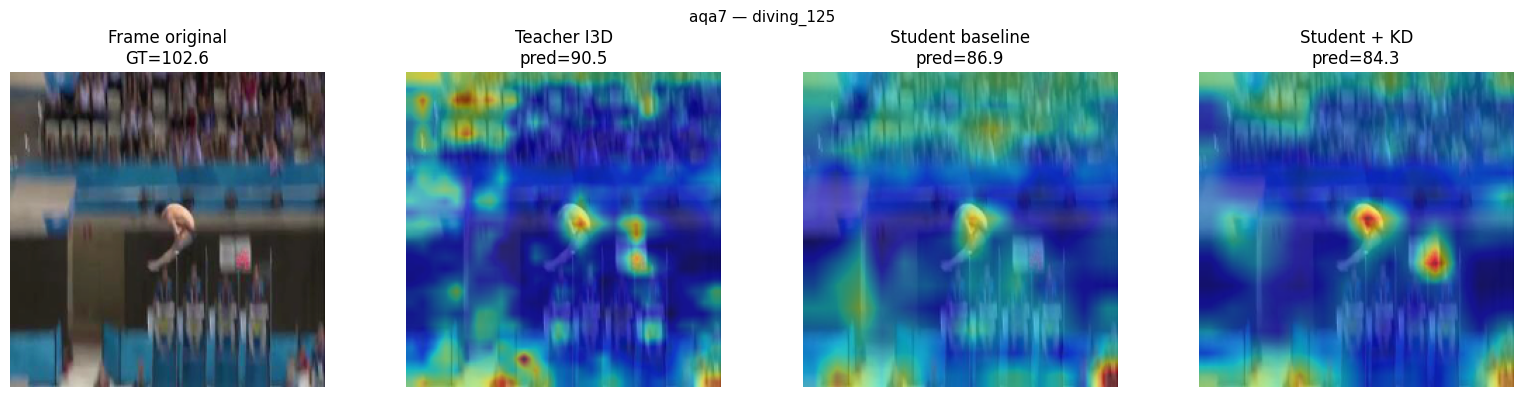
\includegraphics[width=0.85\textwidth]{figs/Resultados/gradcam_aqa7_diving.png} \\
        {\footnotesize (a) AQA-7 -- clavado (\textit{diving\_125})} \\[0.4em]
        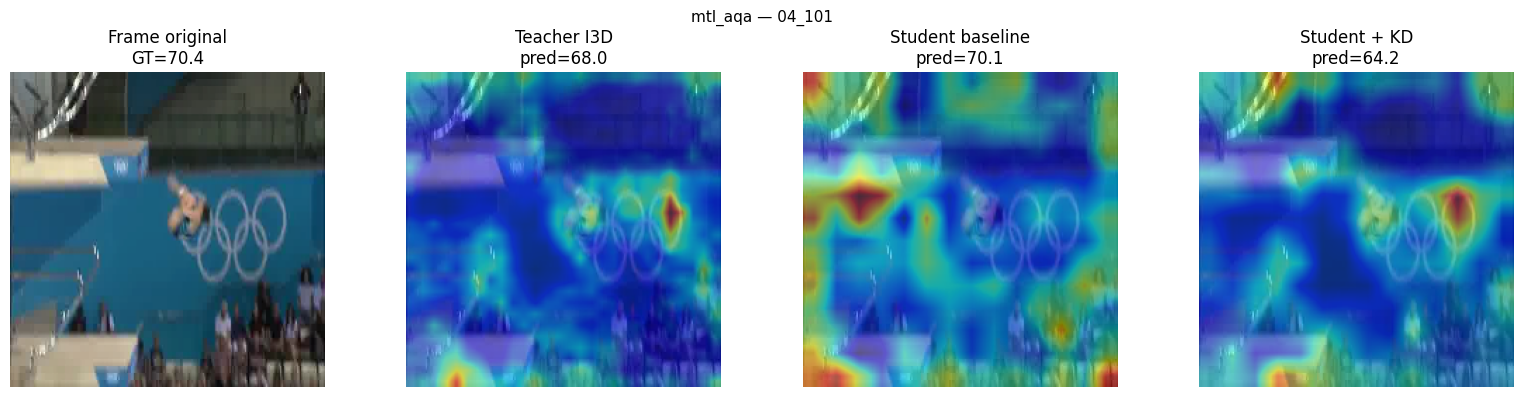
\includegraphics[width=0.85\textwidth]{figs/Resultados/gradcam_mtl_aqa.png} \\
        {\footnotesize (b) MTL-AQA -- clavado (04\_101)} \\[0.4em]
        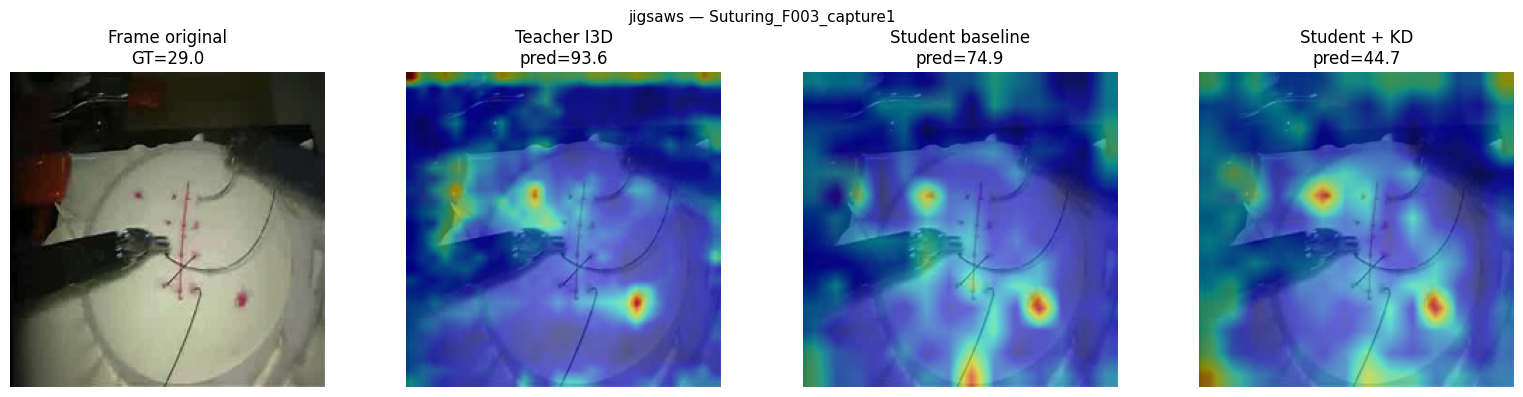
\includegraphics[width=0.85\textwidth]{figs/Resultados/gradcam_jigsaws_suturing.png} \\
        {\footnotesize (c) JIGSAWS -- \textit{Suturing} (F003, capture1)} \\
    \end{tabular}
    \caption{Mapas de atención Grad-CAM para Teacher (\ac{I3D}), \textit{pipeline} liviano y variante \textit{+~KD} en los tres dominios evaluados. En deportes, el \textit{Teacher} concentra la atención sobre el cuerpo del atleta durante la fase clave del movimiento; en cirugía, todos los modelos convergen sobre las manos y los instrumentos.}
    \label{fig:gradcam}
\end{figure}

La inspección visual muestra que el \textit{Teacher} \ac{I3D} concentra su atención sobre el cuerpo del atleta y las extremidades durante la fase clave del movimiento. El \textit{pipeline} liviano sin destilación reproduce patrones cualitativamente similares, lo cual es coherente con la pequeña brecha cuantitativa de \ac{SRCC}. En JIGSAWS las atenciones convergen sobre las manos del cirujano y los instrumentos, indicando que los modelos aprenden a localizar la región relevante incluso en un dominio radicalmente distinto al de pre-entrenamiento.
 %Inserta el capítulo 4
\chapter{Conclusiones y Trabajos Futuros}\label{chap:conclusiones}

En este capítulo se presentan las conclusiones obtenidas a partir del desarrollo de la presente tesis, organizadas conforme a los objetivos específicos definidos en el Capítulo~1. Se describen los principales problemas encontrados, se identifican limitaciones del trabajo y se proponen líneas de investigación futura.

\section{Conclusiones por Objetivos Específicos}

\begin{itemize}
    \item \textbf{OE1 — Estado del arte:} Se realizó un análisis crítico de los enfoques actuales en \ac{AQA} y de las técnicas de compresión y destilación aplicadas a video. Se identificó que la literatura previa parte de la suposición implícita de una brecha sustancial entre \textit{Teachers} 3D pesados y \textit{Students} livianos, suposición formulada en un contexto donde los pesos preentrenados, los optimizadores y las prácticas de entrenamiento eran menos maduros.

    \item \textbf{OE2 — Pipeline reproducible:} Se construyó un \textit{pipeline} liviano basado en TSM-MobileNetV2 y MobileNetV3, inicializados con pesos preentrenados de ImageNet y entrenados con prácticas modernas (AdamW, programación cosenoidal, precisión mixta, acumulación de gradientes). El \textit{pipeline} es reproducible (semillas explícitas, configuraciones \texttt{YAML}) y se aplica de forma uniforme a tres dominios.

    \item \textbf{OE3 — Cuantificación de la brecha:} En AQA-7, el \textit{pipeline} liviano alcanza \ac{SRCC} de $0.9021 \pm 0.005$ (TSM-MobileNetV2) y $0.8907 \pm 0.005$ (MobileNetV3) sobre tres semillas, frente a $0.9052$ (\ac{I3D}) y $0.9158$ (SlowFast-R50). La brecha respecto a ambos \textit{Teachers} 3D es menor a $0.025$ \ac{SRCC} y se mantiene robusta entre semillas. En MTL-AQA y JIGSAWS la brecha es similar ($<0.01$ \ac{SRCC}), confirmando que el resultado es estable en dominios de naturaleza distinta.

    \item \textbf{OE4 — Ablaciones de componentes:} El preentrenamiento ImageNet aporta $\sim 0.031$ \ac{SRCC} sobre el backbone aleatorio (E6), constituyendo el componente más importante del \textit{pipeline}. El módulo Temporal Shift (\ac{TSM}) aporta $\sim 0.010$ \ac{SRCC} adicional (E7), beneficio modesto pero positivo. El \textit{pipeline} se sostiene en dos componentes identificables: preentrenamiento ($\sim 3$ puntos) y modelado temporal eficiente ($\sim 1$ punto).

    \item \textbf{OE5 — Eficiencia computacional:} Los \textit{Students} usan menos del $9\%$ de los \ac{FLOPs} del \textit{Teacher} \ac{I3D} (TSM-MobileNetV2: 20.0~G; MobileNetV3: 14.3~G; vs 228.3~G del \ac{I3D}), con parámetros aproximadamente $10\times$ menores y latencia de inferencia entre $2.5$ y $3.4\times$ menor. MobileNetV3 alcanza 39.9~ms por clip de 64 \textit{frames} en RTX 3060 Mobile, habilitando aplicaciones en tiempo real.

    \item \textbf{OE6 — Límites de aplicabilidad:} La transferencia cruzada \textit{zero-shot} obtiene \ac{SRCC} parcial entre dominios deportivos ($\sim 0.55$) y fracasa entre deporte y cirugía. La introducción de \textit{Test-Time Adaptation} por recalibración de BatchNorm (primera aplicación documentada de TTA a \ac{AQA}) mejora 11 de 12 configuraciones evaluadas, con ganancias particularmente notables en pares de mayor \textit{domain shift} (hasta $+0.12$ \ac{SRCC}), sin requerir reentrenamiento ni etiquetas del dominio \textit{target}. El análisis marginal de la destilación muestra que, sobre la línea base liviana fuerte, la \ac{KD} no aporta valor consistente: sólo 1 de 6 configuraciones mejora con \ac{KD}, lo que delimita el alcance del \textit{pipeline} y replantea el rol de la destilación en \ac{AQA} eficiente.
\end{itemize}

\section{Conclusión General}

La presente tesis sostiene tres conclusiones positivas y empíricamente respaldadas:

\textbf{Primero}, un \textit{pipeline} moderno de \textit{Students} livianos (TSM-MobileNetV2 y MobileNetV3 con preentrenamiento ImageNet, AdamW, cosine annealing, AMP y \textit{gradient accumulation}) alcanza \ac{SRCC} a menos de $0.025$ del \textit{Teacher} 3D moderno SlowFast-R50, y a menos de $0.015$ del \ac{I3D}, utilizando el $9\%$ de sus \ac{FLOPs}. Este resultado es estable entre semillas (std $\approx 0.005$) y reproducible en tres dominios (AQA-7, MTL-AQA, JIGSAWS).

\textbf{Segundo}, las ablaciones identifican los componentes responsables del rendimiento del \textit{pipeline}: el preentrenamiento ImageNet (E6, $\sim 3$ puntos de \ac{SRCC}) y el módulo Temporal Shift (E7, $\sim 1$ punto adicional). Esto convierte el \textit{pipeline} en una propuesta interpretable: su aporte no es un efecto agregado opaco, sino la contribución cuantificable de elementos identificables.

\textbf{Tercero}, el análisis marginal de la destilación de conocimiento muestra que, cuando el \textit{Student} se entrena con un \textit{pipeline} fuerte, la \ac{KD} no aporta valor consistente y puede incluso degradar el rendimiento; en contraste, la incorporación de \textit{Test-Time Adaptation} por recalibración de BatchNorm mejora la transferencia cruzada en 11 de 12 configuraciones evaluadas, constituyendo la primera aplicación documentada de TTA a \ac{AQA}. Esto cuestiona la premisa heredada de la literatura previa---según la cual el cierre de brecha entre \textit{Teacher} y \textit{Student} requiere destilación---y replantea la prioridad de futuras propuestas en \ac{AQA} eficiente hacia mecanismos sin gradiente como TTA.

\textbf{Cuarto}, la comparación con el estado del arte sitúa el \textit{pipeline} propuesto por encima de varios métodos representativos del campo en AQA-7 (USDL, GAKD, CoRe, TSA-Net, HGCN) usando aproximadamente el $9\%$ de sus \ac{FLOPs}. En MTL-AQA el \textit{pipeline} queda 7--8 puntos por debajo del SOTA, brecha aceptable dado el ahorro computacional y el contexto de despliegue embebido en el que se ubica la propuesta.

En conjunto, la tesis entrega un \textit{pipeline} liviano reproducible, eficiente, competitivo con métodos del estado del arte en su régimen de costo, y con sus componentes, sus límites de aplicabilidad y un mecanismo complementario de adaptación cross-domain claramente delimitados.

\section{Limitaciones del trabajo}

Para una interpretación honesta del aporte se enumeran a continuación las principales limitaciones, cada una de las cuales abre una línea concreta de trabajo futuro:

\begin{itemize}
    \item \textbf{Réplicas por semilla limitadas a un dataset.} Las réplicas con tres semillas se ejecutaron únicamente sobre AQA-7 (dataset principal). En MTL-AQA y JIGSAWS los resultados se reportan con semilla 42 por costo computacional acumulado. Los hallazgos cuantitativos en esos dos dominios deben leerse considerando esta limitación.

    \item \textbf{Sin validación en hardware embebido real.} La medición de eficiencia se realizó en RTX 3060 Mobile como aproximación a hardware de bajo costo, pero no se ejecutó el modelo en plataformas embebidas reales (Jetson Nano, dispositivos móviles). La validación en tales plataformas, incluyendo consumo energético y memoria de \textit{runtime}, queda como trabajo futuro.

    \item \textbf{Restricciones de memoria que afectaron el régimen de entrenamiento.} El \textit{batch size} físico de 1--2 (impuesto por los 6~GB de \ac{VRAM}) hizo necesario congelar las estadísticas de \textit{BatchNorm} del \textit{Student} durante el entrenamiento con \ac{KD}. Aunque preserva la estabilidad numérica, este procedimiento podría sesgar la evaluación del análisis marginal de \ac{KD} frente a configuraciones con mayor capacidad de hardware.

    \item \textbf{Generalización cross-domain limitada al régimen \textit{zero-shot}.} La transferencia AQA-7 $\to$ JIGSAWS se evaluó sin \textit{fine-tuning}; el resultado negativo no descarta que la destilación o el \textit{pipeline} puedan funcionar tras adaptación de dominio.

    \item \textbf{Subconjunto del paisaje de Students livianos.} Se evaluaron dos arquitecturas (TSM-MobileNetV2 y MobileNetV3); la generalización del hallazgo a otras familias (EfficientNet-Video, X3D-S, MoViNet) requiere validación adicional.
\end{itemize}

\section{Problemas encontrados}

\begin{itemize}
    \item \textbf{Desbalance de clases y distribución de etiquetas:} los datasets empleados presentan concentraciones en rangos medios de puntuación. Esto afectó la capacidad del modelo para distinguir los extremos del espectro de calidad.

    \item \textbf{Variabilidad en las condiciones visuales:} se observaron casos con iluminación deficiente, ángulos de cámara extremos o ruido visual.

    \item \textbf{Limitaciones del hardware de entrenamiento:} la ejecución de modelos 3D (\ac{I3D}, SlowFast) y el cálculo de pérdidas de destilación implicaron una alta demanda de memoria. Esto obligó a reducir tamaños de \textit{batch} y emplear acumulación de gradientes.

    \item \textbf{Ausencia de benchmarks estandarizados para AQA eficiente:} la falta de protocolos unificados dificultó la comparación directa con trabajos previos, haciendo necesario definir un \textit{pipeline} experimental propio.
\end{itemize}

\section{Trabajos futuros}

\begin{itemize}
    \item \textbf{Score Distribution Learning} adaptado al \textit{pipeline} liviano: experimentos preliminares de variantes de regresión distribucional (\textit{Uncertainty-aware Score Distribution Learning}, Tang et al. 2020) mostraron mejoras de hasta $+0.053$ \ac{SRCC} en TSM-MobileNetV2 + JIGSAWS sobre la línea base liviana, sugiriendo que el reformulado del objetivo de regresión es una dirección promisoria.

    \item \textbf{Adaptación de dominio} para resolver el fracaso de transferencia AQA-7 $\to$ JIGSAWS: explorar técnicas como CORAL, MMD o adaptación adversarial.

    \item \textbf{Réplicas por semilla en MTL-AQA y JIGSAWS} para extender la robustez estadística más allá del dataset principal.

    \item \textbf{Implementación en dispositivos reales} (Jetson Nano, móviles) midiendo consumo energético, latencia real y memoria de \textit{runtime}.

    \item \textbf{Aplicación en nuevos dominios} (rehabilitación física, educación física, evaluación de gestos motores en condiciones clínicas).

    \item \textbf{Análisis explicable de decisiones} mediante técnicas de interpretabilidad para facilitar adopción en entornos sensibles como análisis clínico o juicio técnico profesional.
\end{itemize}
 %Inserta el capítulo 5

%%%%%%%%%%%%%%%%%%%%%%%%%%%%%%%%%%%%%%%%%%%%%%%%%%%%%%%%%%%%%%%%%%%%%%

\bibliographystyle{apalike}

\bibliography{Bibliog}
\addcontentsline{toc}{chapter}{Bibliografía}
\end{document}
